\documentclass[xcolor=dvipsnames, handout]{beamer}

% 1. PREÁMBULO: Configuraciones Globales
\usetheme{Madrid}
\usepackage[utf8]{inputenc}
\usepackage[spanish, es-tabla]{babel} % es-tabla para que diga Tabla y no Cuadro
\usepackage{amsmath, amssymb}
\usepackage{diagbox}
\usepackage{multirow}
\usepackage{tikz}

% 2. CONFIGURACIÓN DE TIKZ (Debe ir en el preámbulo)
\usetikzlibrary{arrows.meta, positioning, calc}
\tikzset{
    state/.style={circle, draw=black, thick, minimum size=1.1cm, font=\bfseries},
    alc/.style={state, fill=Emerald!20, text=Emerald!70!black},
    baj/.style={state, fill=Maroon!20, text=Maroon!70!black},
    est/.style={state, fill=Gray!20, text=Gray!70!black},
    trans/.style={->, >={Stealth[scale=1.0]}, thick, black!70, shorten >=1pt},
    val/.style={font=\tiny\bfseries, text=blue!80!black, yshift=2mm}
}

\title{Toma de Decisiones Secuenciales \\ y Aprendizaje por Refuerzo}
\author{Daniela Pucci de Farias}
\institute{Universidad Torcuato Di Tella}
\date{Modulo 3: Aprendizaje por Refuerzo}

% 3. PERSONALIZACIÓN DEL FOOTER (Muestra únicamente: Módulo | Páginas con margen izquierdo)
\setbeamertemplate{footline}{
  \leavevmode%
  \hbox{%
  % Bloque 1 (Izquierda/Centro): Nombre del Módulo con más espacio al borde (leftskip)
  \begin{beamercolorbox}[wd=.8\paperwidth,ht=2.25ex,dp=1ex,leftskip=4ex,left]{title in head/foot}%
    \usebeamerfont{title in head/foot}\hspace*{2ex} \insertdate
  \end{beamercolorbox}%
  % Bloque 2 (Derecha): Numeración de Páginas
  \begin{beamercolorbox}[wd=.2\paperwidth,ht=2.25ex,dp=1ex,right]{date in head/foot}%
    \usebeamerfont{date in head/foot}
    \insertframenumber{} / \inserttotalframenumber\hspace*{2ex} 
  \end{beamercolorbox}}%
  \vbox{}%
}

\begin{document}

\frame{\titlepage}

% --- SLIDE: REPASO MDP ---
\begin{frame}{Repaso MDPs}
En el m\'odulo anterior, estudiamos el marco de MDPs para resolver problemas de toma de decisioes secuenciales. La clave fue la \textbf{Ecuaci\'on de Bellman}:
\[ V^*(s) = \max_{a \in A} \left\{ r(s,a) + \alpha \sum_{s'} P(s,a,s') V^*(s') \right\} \]

\begin{itemize}
    \item \textbf{Iteraci\'on de Valor:} Actualiza valores hasta converger.
    \item \textbf{Iteraci\'on de Pol\'itica:} Alterna entre evaluar $V_u$  y mejorar $u$.
\end{itemize}

\end{frame}

% --- SLIDE: MDPs EN EL MUNDO REAL ---
\begin{frame}{¿Por qu\'e no siempre podemos usar MDPs cl\'asicos?}

\begin{itemize}
    \item Si gestionamos un inventario de 100 productos, \textquestiondown c\'omo ser\'a el espacio de estados? \textquestiondown Cu\'anto tiempo y espacio se necesitar\'a para calcular y almacenar $V^*$?
    
    \item<2-> En un e-commerce (precificaci\'on), no conocemos la probabilidad real de que un cliente acepte un precio, y puede cambiar con el tiempo. 
    
    \item<3-> En la gesti\'on de relaciones con clientes (CRM), el estado emocional del cliente no se ve. Solo tenemos indicadores ruidosos (clics, quejas).
\end{itemize}


\end{frame}

% --- SLIDE: HACIA EL REINFORCEMENT LEARNING ---
\begin{frame}{Desaf\'ios y Soluciones}

        \begin{block}{1. La Maldici\'on de la Dimensionalidad}
            \small Crecimiento exponencial en el n\'umero  de estados y/o acciones.

            \vspace{0.2cm}
           \visible<2->{ \textbf{\textcolor{red}{Soluci\'on: Generalizaci\'on}} \\
            En lugar de tablas, empleamos arquitecturas de aproximaci\'on (como redes neuronales) para representar las funci\'ones de valor y/o pol\'itica.}
        \end{block}
        \begin{block}{2. Informaci\'on Parcial}
            \small No conocemos $P(s'|s,a)$ ni $r(s,a)$.

            \vspace{0.2cm}
\visible<3->{
            \textbf{\textcolor{red}{Soluci\'on: Aprendizaje}} \\
            El agente debe interactuar con el entorno y aprender de la experiencia (\textbf{RL}).}
        \end{block}
        
        \begin{block}{3. Estados Ocultos}
            \small El estado real no es visible, solo observacions relacionadas.

            \vspace{0.2cm}
\visible<4->{
            \textbf{\textcolor{red}{Soluci\'on: POMDPs}} \\
            Actuar en el espacio de probabilidades de estados.}
        \end{block}



\end{frame}

\begin{frame}{Desafío: Incertidumbre y Datos}
\begin{itemize}
    \item Hasta ahora, dependíamos de $P$ y $r$. ¿Qué sucede cuando las reglas del ambiente son desconocidas o demasiado complejas para modelar?
    
    \item<2-> \textbf{La Propuesta:} Aprender la política óptima directamente a partir de la \textbf{interacción} con el ambiente.
\end{itemize}

\vspace{-0.2cm}
\begin{center}
\mode<beamer>{
\only<2,3>{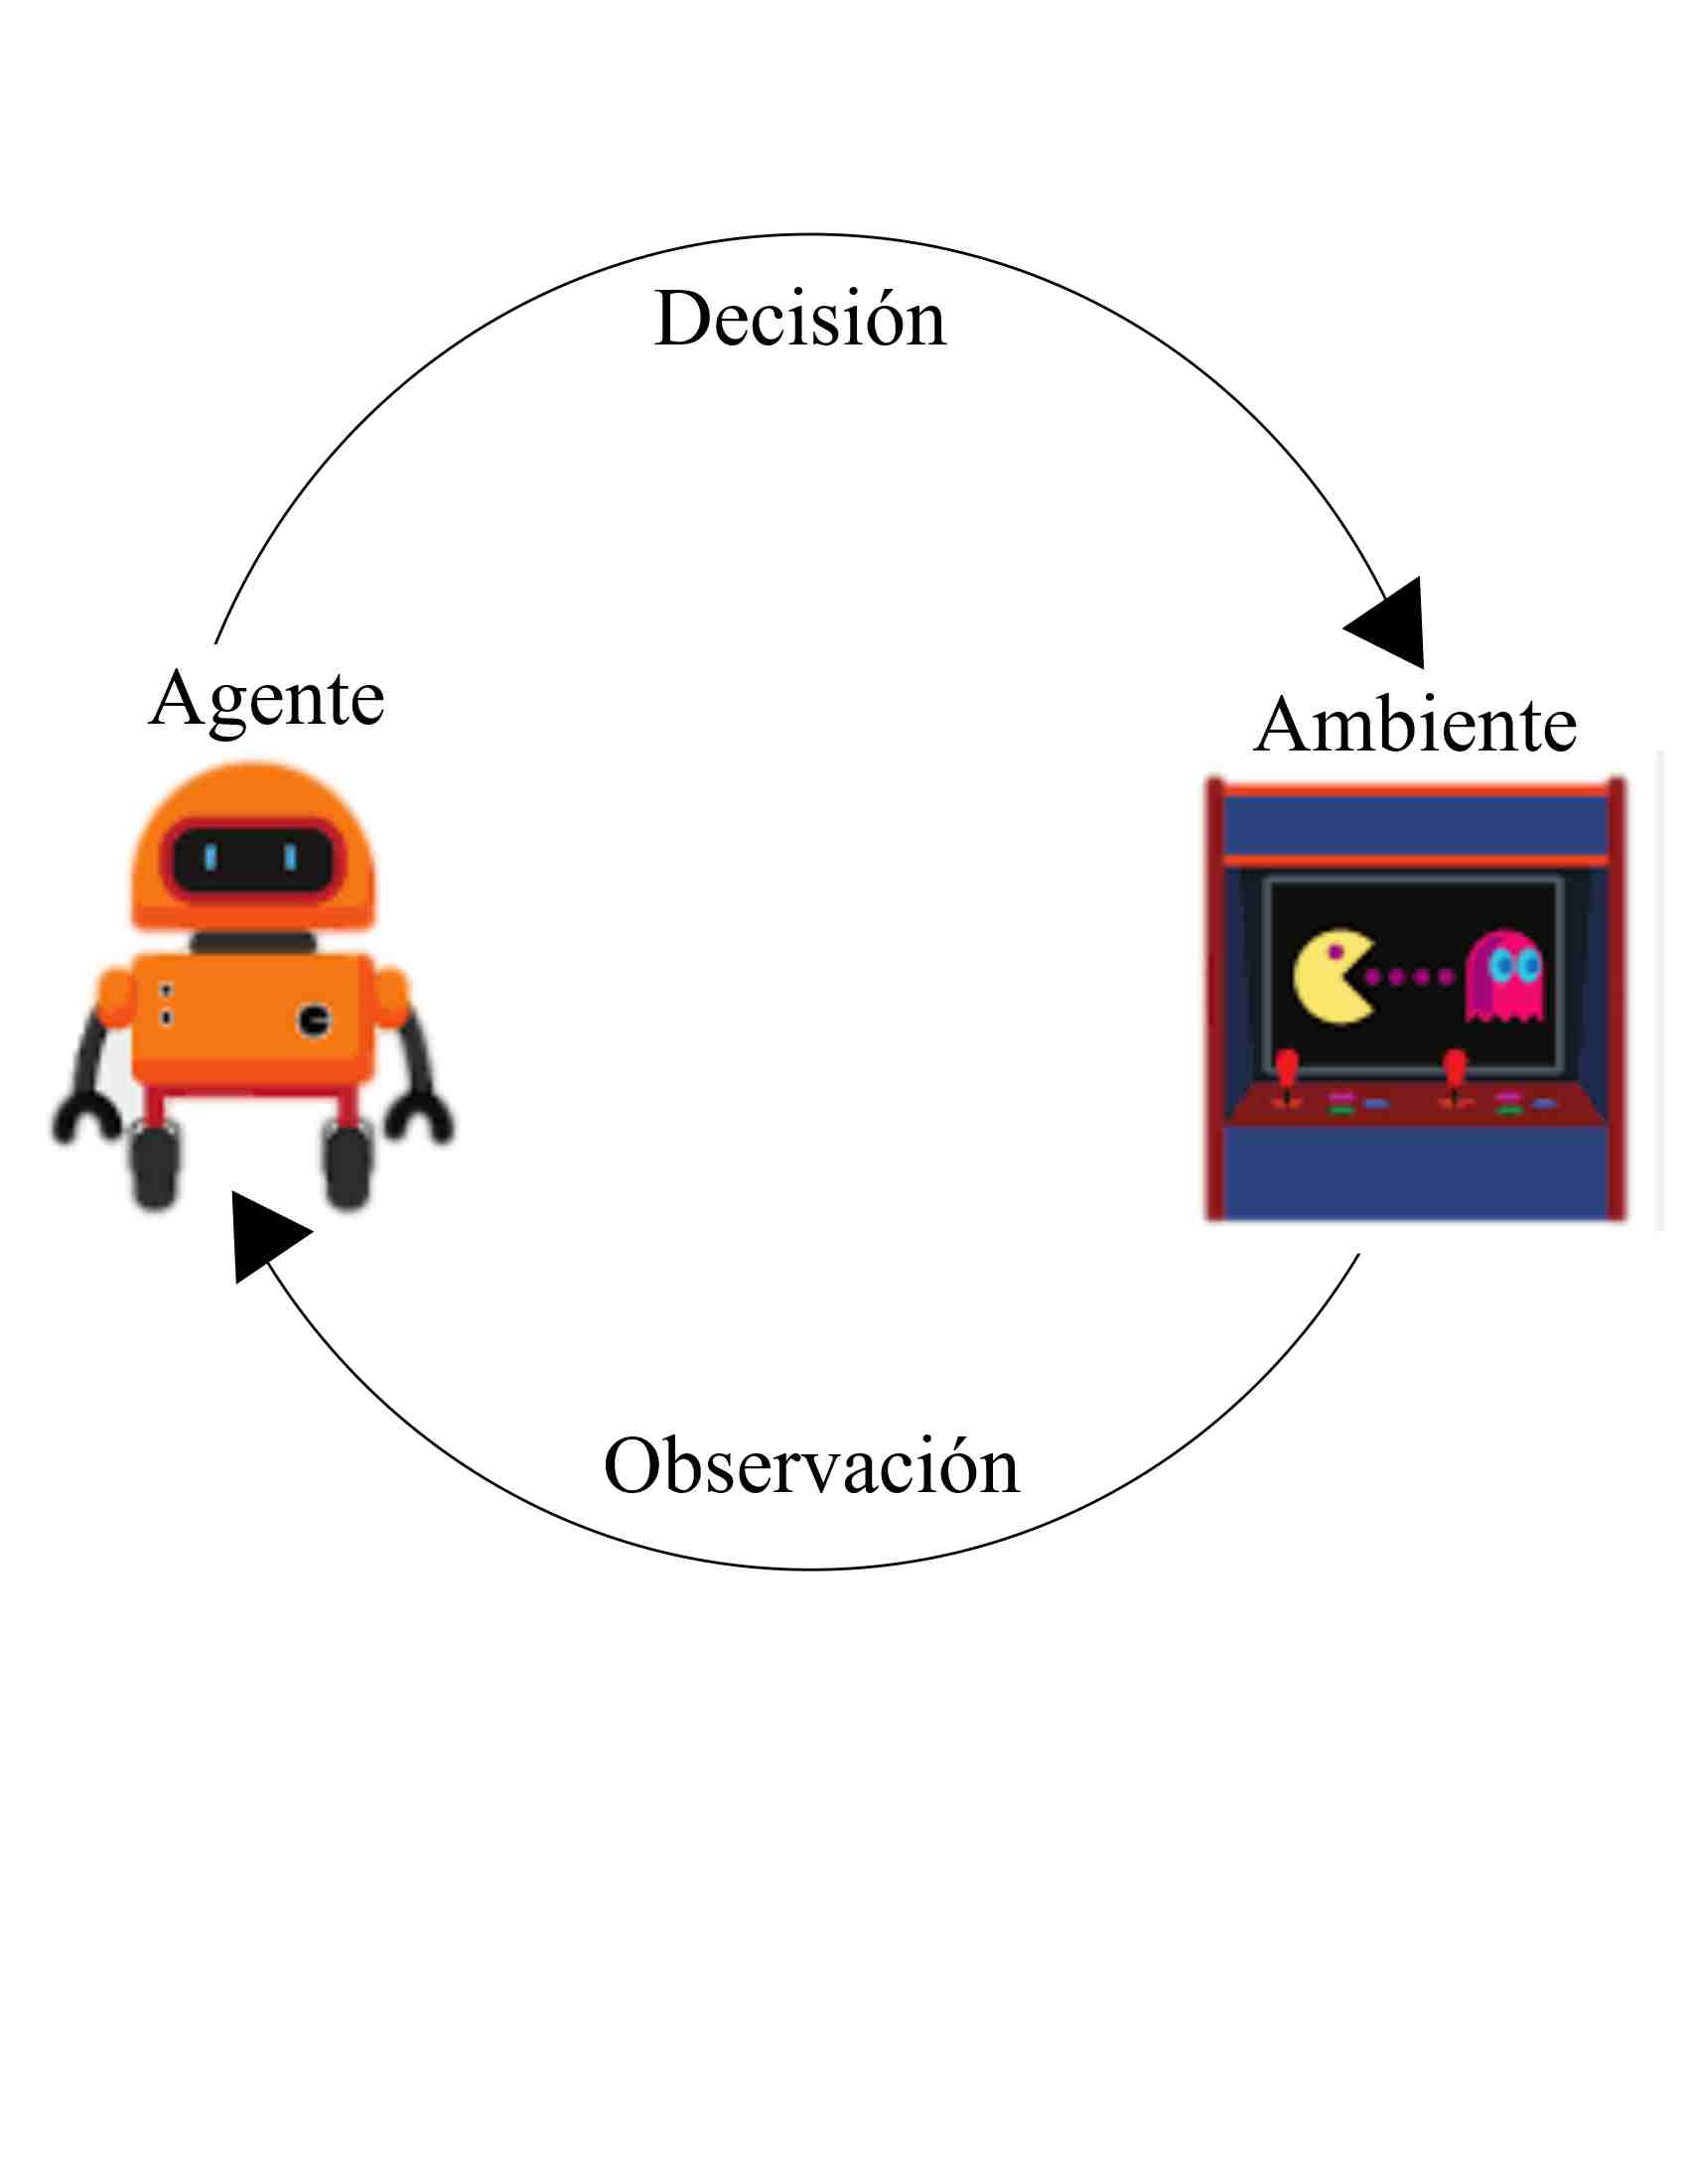
\includegraphics[width=0.35\textwidth]{../Images/LearningCycle/RL2.jpg}} 
\only<4>{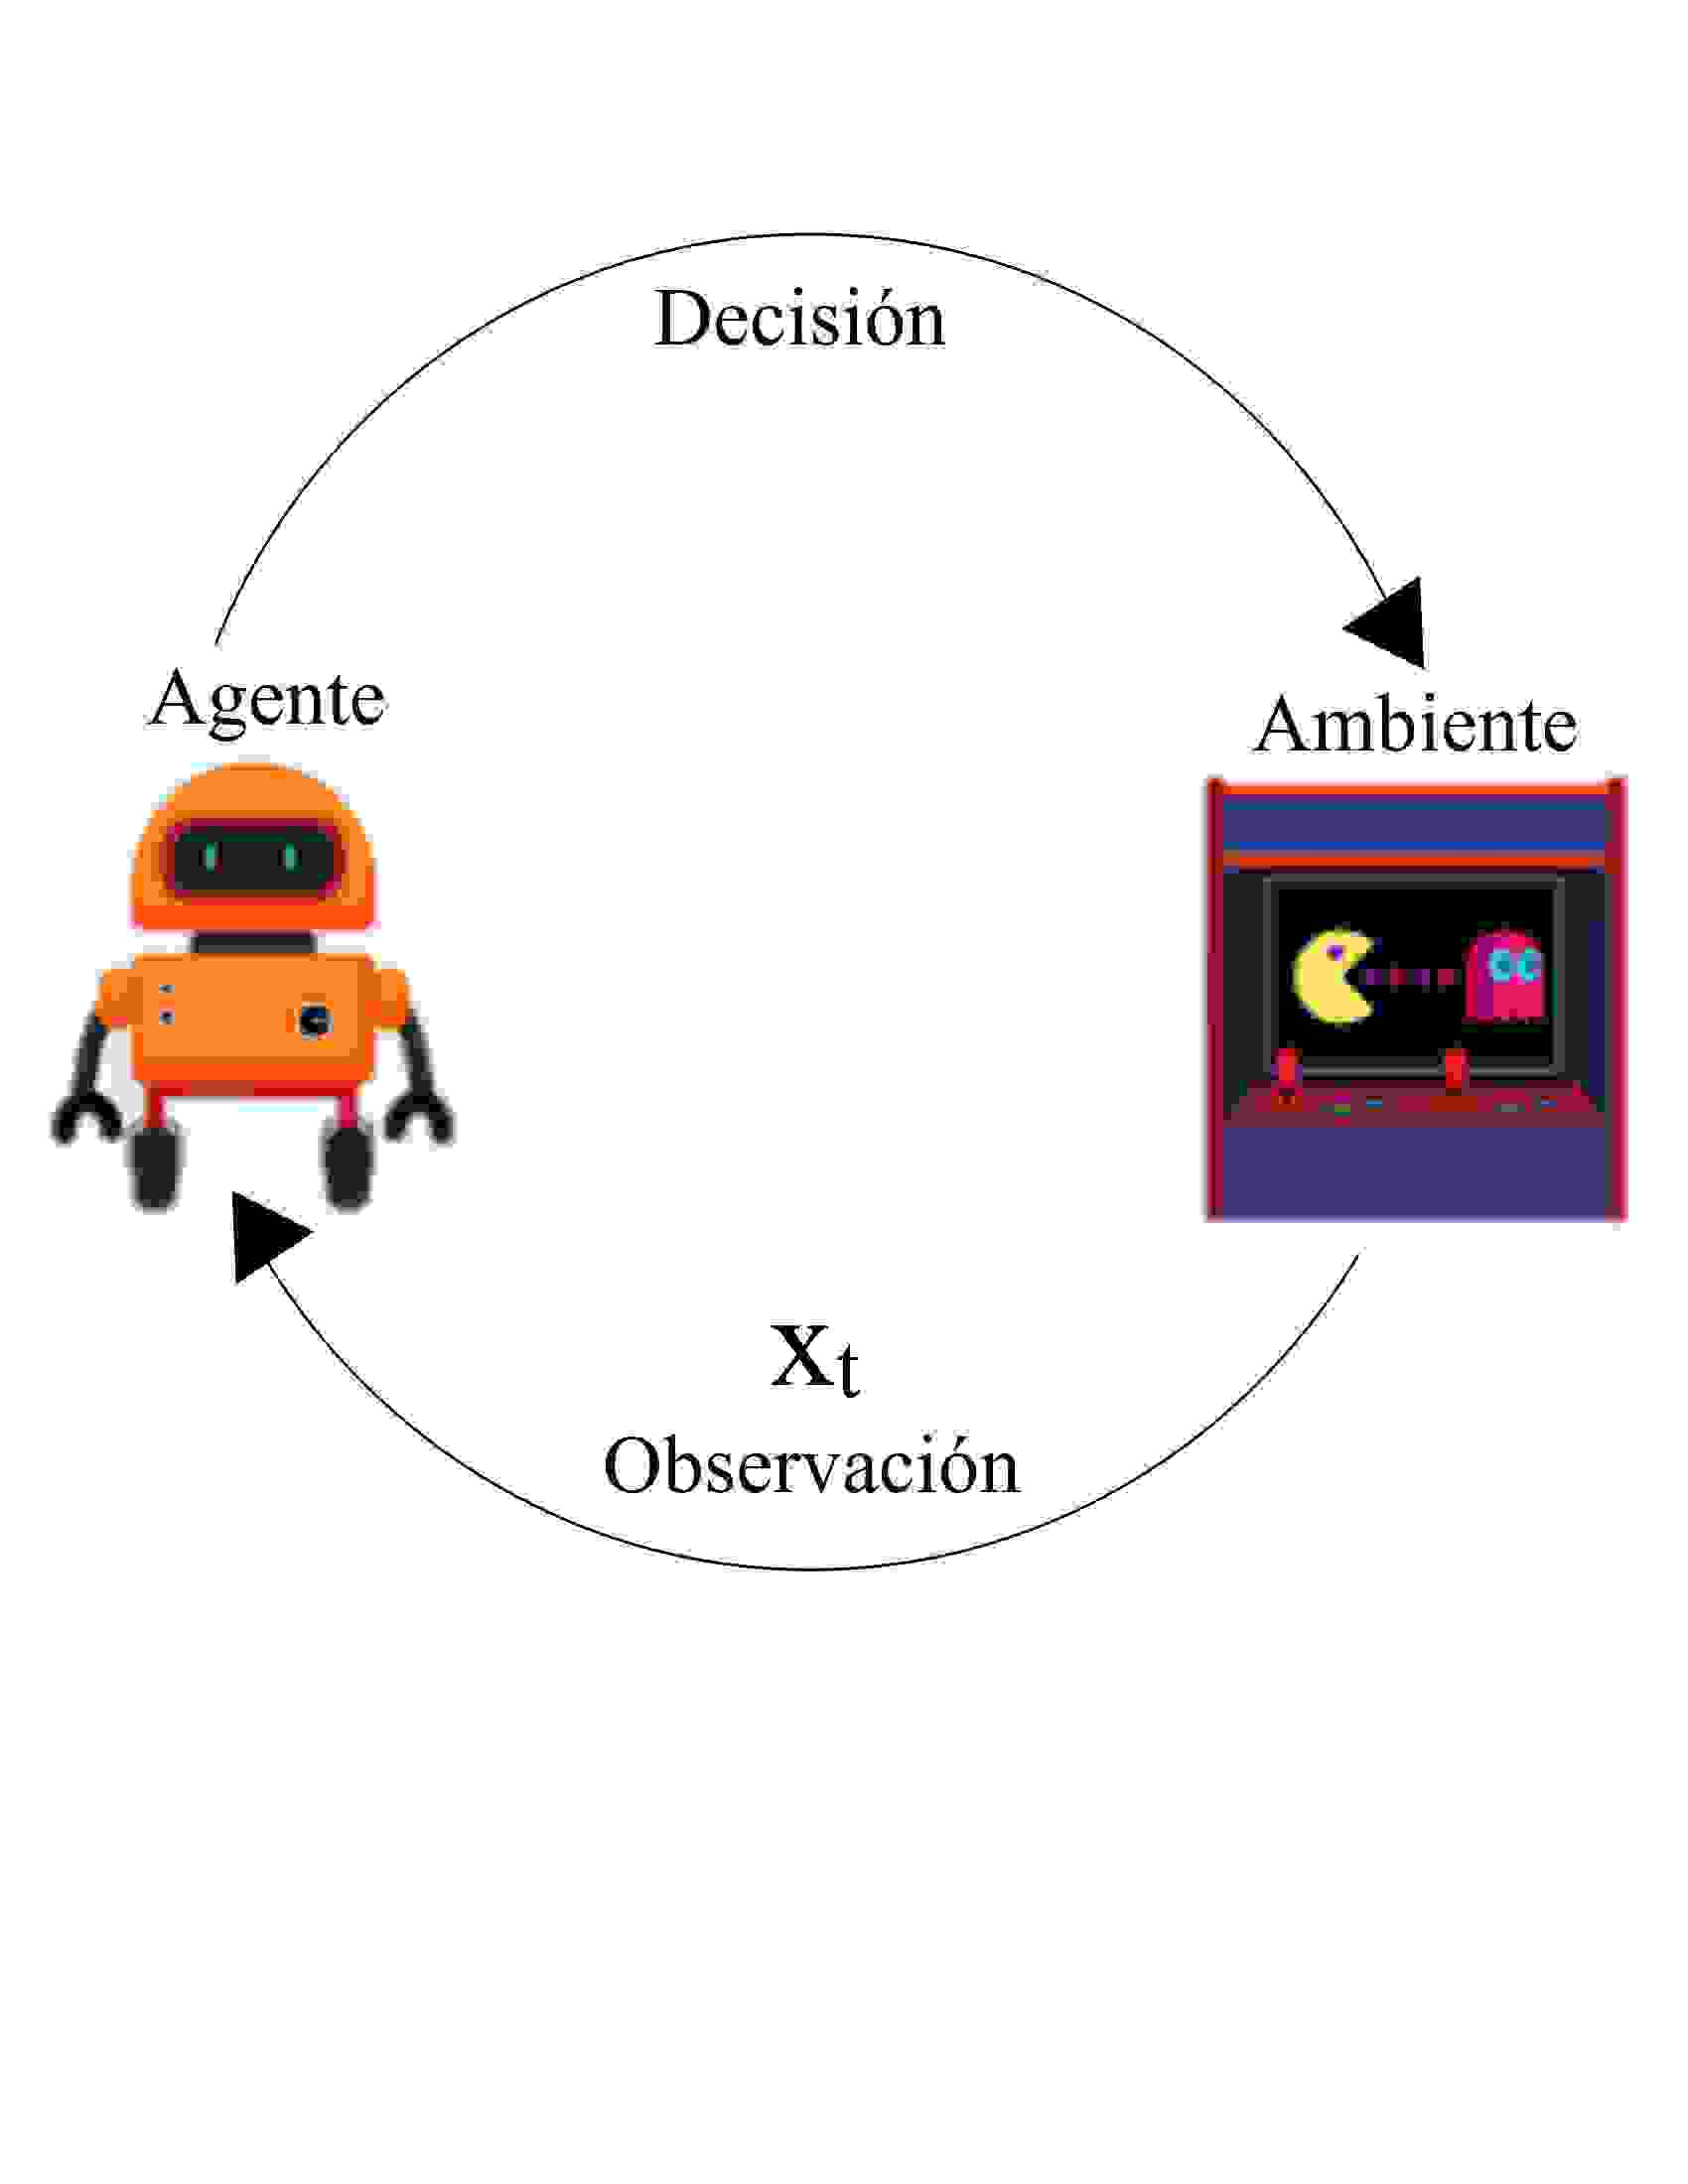
\includegraphics[width=0.35\textwidth]{../Images/LearningCycle/LearningCycle1.jpg}}  
\only<5>{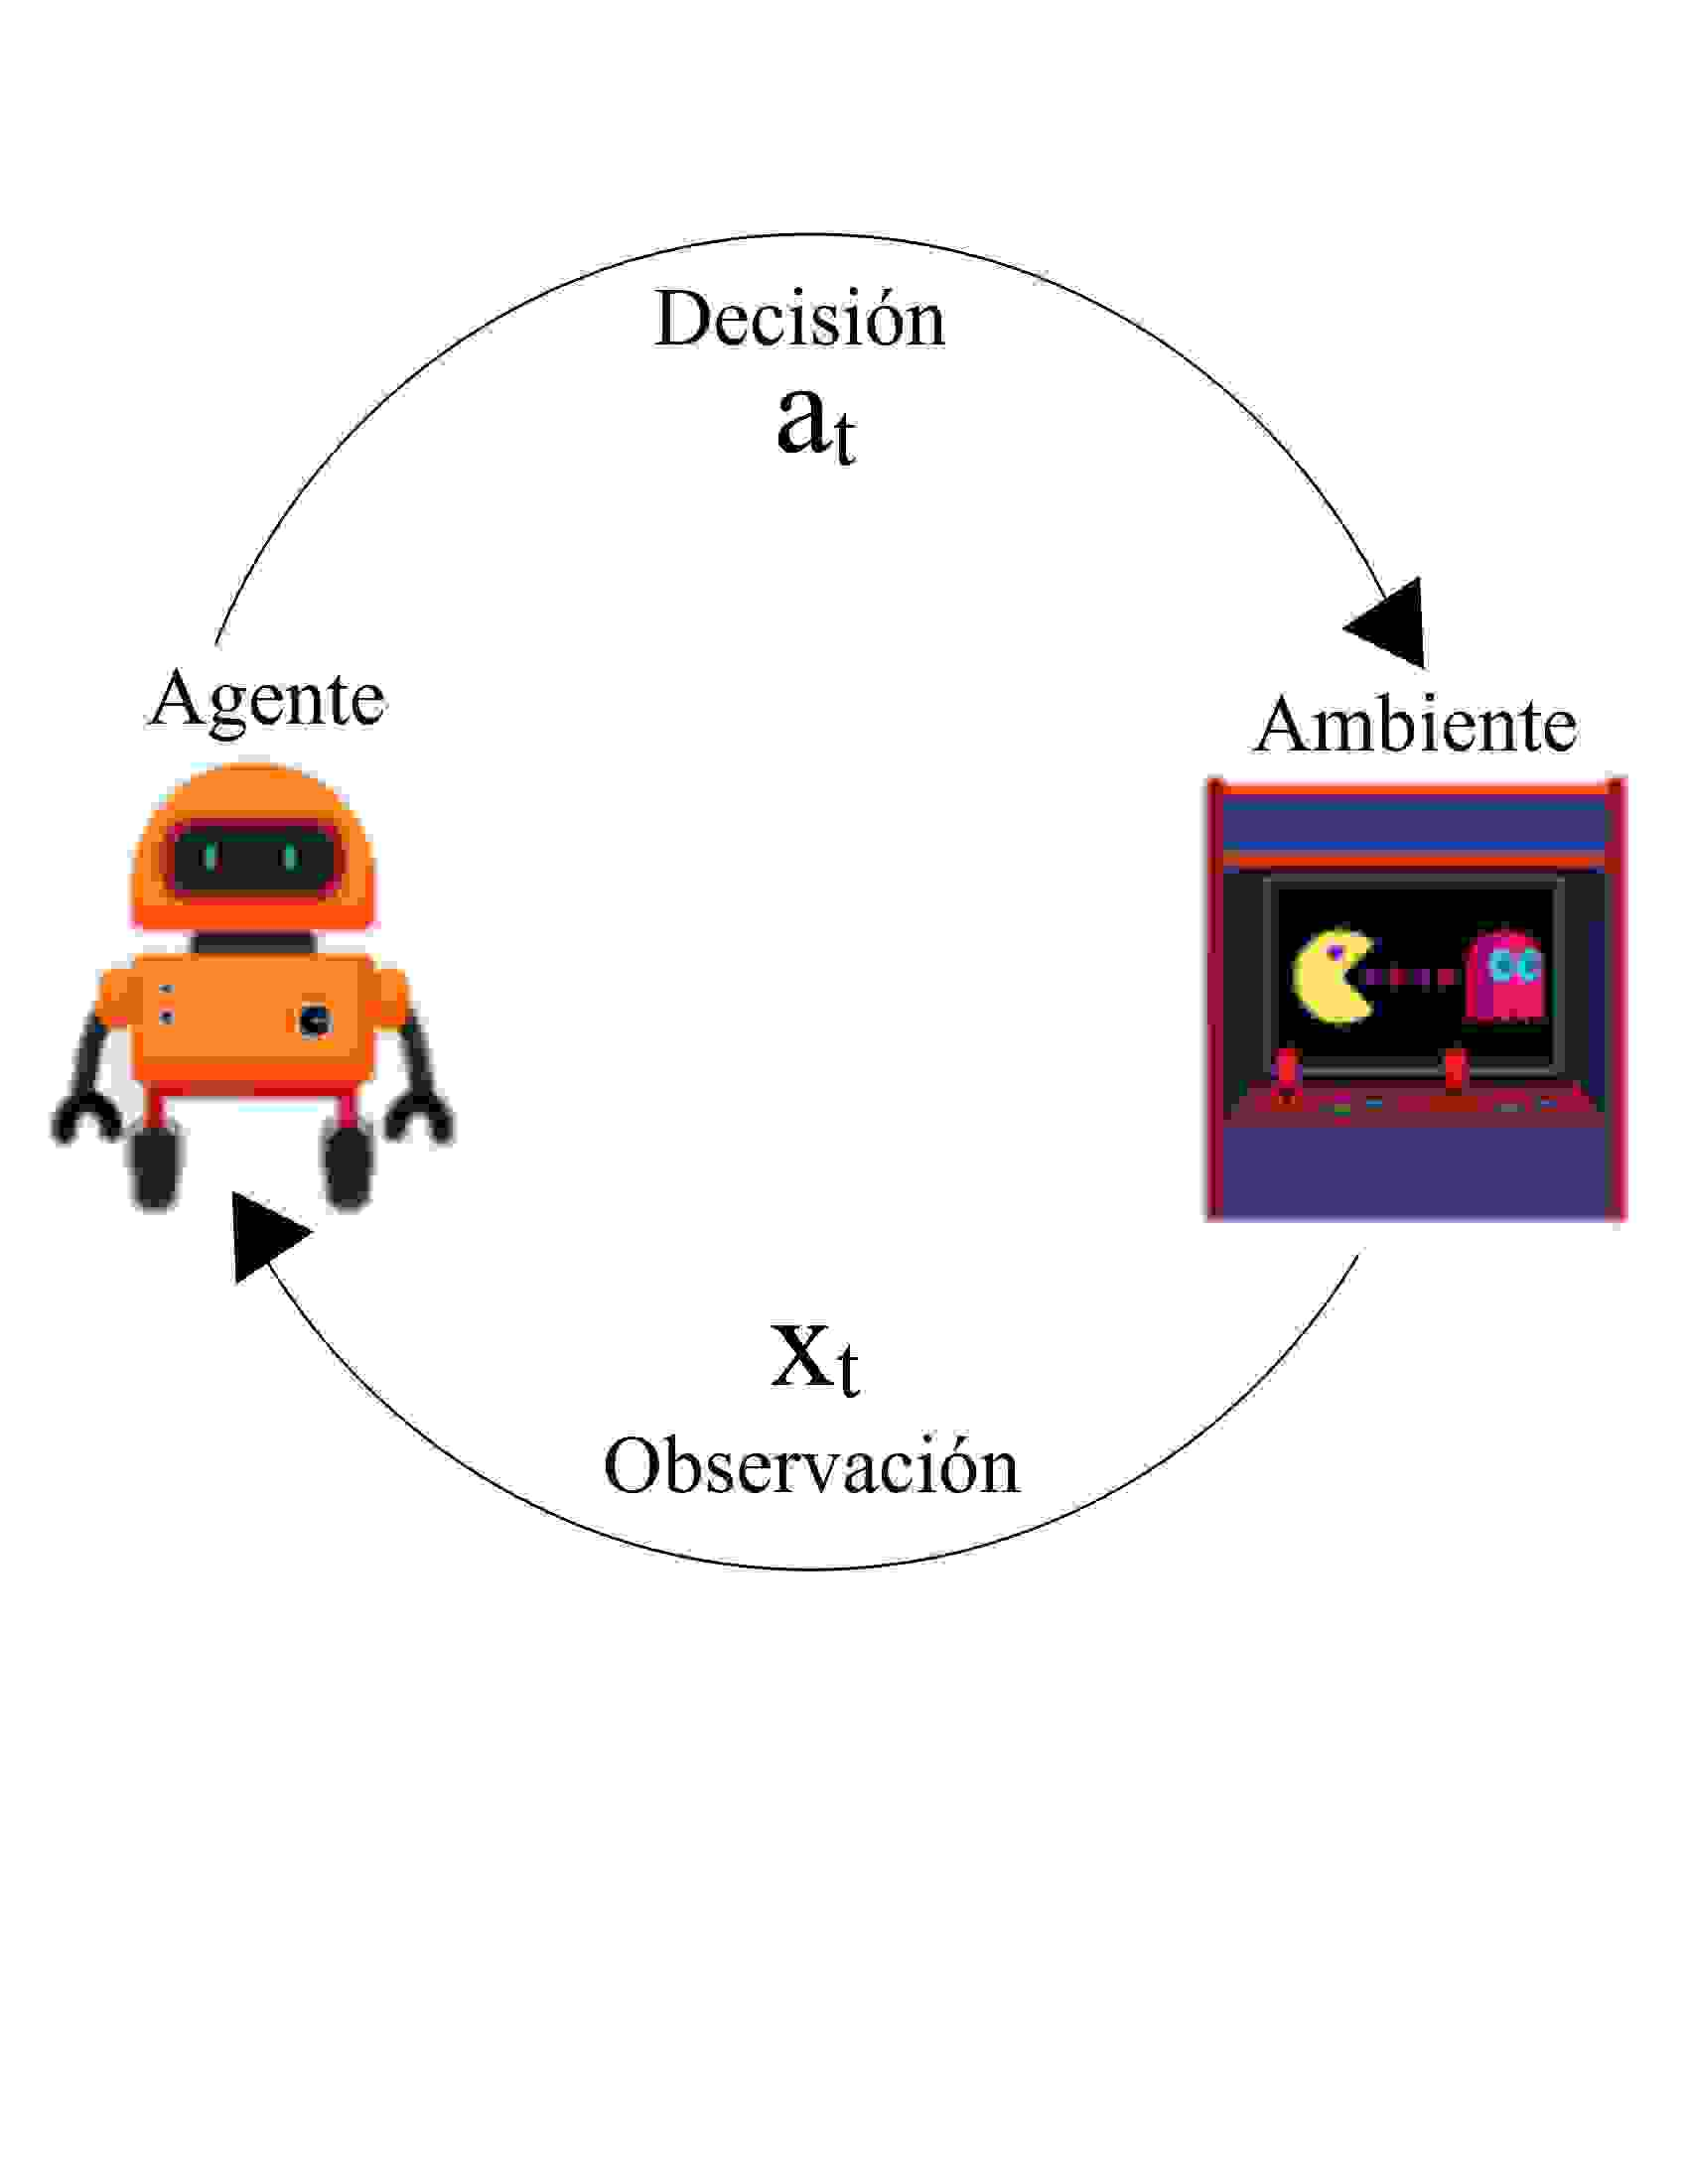
\includegraphics[width=0.35\textwidth]{../Images/LearningCycle/LearningCycle2.jpg}} }
\only<6->{\includegraphics[width=0.35\textwidth]{../Images/LearningCycle/LearningCycle3.jpg}} 
\end{center}
\end{frame}

\begin{frame}{Desafío: Incertidumbre y Datos}
\begin{itemize}
    \item \textbf{¿Con qué datos contamos?} 
    \begin{itemize}
        \item<2-> \textbf{Trayectorias:} Secuencias temporales de estados y acciones.
        \begin{itemize}
            \item<3-> Única (horizonte largo): $(x_0, a_0, r_0, x_1, a_1, r_1, \dots)$
            \item<4-> Múltiples (episodios): $\{(x_0^i, a_0^i, r_0^i, \dots, x_T^i)\}_{i=1}^M$
        \end{itemize}
        \item<5-> \textbf{Tuplas (Transiciones):} Conjuntos de experiencias aisladas $(x, a, r, y)$. 
    \end{itemize}
\item Al contrario del aprendizaje supervisado, no tenemos observaciones de la funci\'on de valor o de la funci\'on pol\'itica.
\end{itemize}
\end{frame}

\begin{frame}{Model-Based vs. Model-Free RL}
\centering
\scalebox{0.7}{
\begin{tikzpicture}[
    node distance=5cm, 
    every node/.style={draw, thick, rounded corners, inner sep=10pt, font=\small, align=center},
    arrow/.style={-stealth, ultra thick}
]
  % Nodos Principales
  \node (data) [fill=gray!10] {Experiencias \\ $ (x^i,a^i,r^i,y^i)$ \\ $i=1,2,\dots,N$};
  \node<2-> (model) [right of=data, fill=blue!5] {Modelo Estimado \\ $\hat P,~\hat r$};
  \node<5-> (V_and_u) [right of=model, fill=green!5] {Funci\'on Valor $\hat V$ \\ Pol\'itica $\hat u$};
  
  % Flujo Model-Based
  % Se añade draw=none para que las etiquetas no tengan recuadro
  \draw<3-> [arrow] (data) -- node[midway, above, font=\scriptsize, draw=none] {Aprendizaje \\ Supervisado} (model);
  \draw<5-> [arrow] (model) -- node[midway, above, font=\scriptsize, draw=none] {Programaci\'on \\ Din\'amica} (V_and_u);
  
  % Flujo Model-Free (RL Directo)
  \draw<6-> [arrow, draw=red] (data) to[bend right=25] 
    node[pos=0.5, below, align=center, font=\small, draw=none] {\textbf{\textcolor{red}{Aprendizaje Por Refuerzo Directo}} \\ \textbf{\textcolor{red}{(Model-Free)}}} (V_and_u);
\end{tikzpicture}}

\begin{itemize}
    \item<2-> \textbf{Enfoque Indirecto (Model-Based):} Construimos un simulador mental del mundo.
    \begin{itemize}
        \item<3-> \textbf{Frecuentista:} $\hat P(x,y) = \frac{|I_{x,y}|}{|I_x|}$. Estimamos probabilidades contando transiciones.
        \item<4-> \textbf{Param\'etrico:} Estimamos leyes f\'isicas o econ\'omicas (ej: volatilidad $\sigma$).
    \end{itemize}
    \item<6-> \textbf{Enfoque Directo (Model-Free):} Saltamos el paso del modelo.
    \begin{itemize}
        \item Aprendemos $\hat V$ o $\hat u$ directamente de los errores de predicci\'on.
    \end{itemize}
\end{itemize}
\end{frame}

% --- SLIDE: ¿CUÁNDO ES ATRACTIVO EL MODELO? ---
\begin{frame}{¿Cu\'ando es atractivo el enfoque Model-Based?}


\begin{itemize}
    \item<1->Cuando el sistema posee una \textbf{estructura} que podemos explotar:
    \begin{itemize}
        \item<2-> \textbf{Modelos Param\'etricos:} Ecuaciones de la f\'isica o econometr\'ia (ej. leyes de Newton, Black-Scholes). Pocos par\'ametros para estimar.
        \item<3-> \textbf{Digital Twins:} R\'eplicas digitales de alta fidelidad de activos f\'isicos (ej. una turbina e\'olica o una red el\'ectrica).
        \item<4-> \textbf{Simuladores Estoc\'asticos:} Modelos de eventos discretos o Monte Carlo para log\'istica y colas.
    \end{itemize}

    \item<5-> \textbf{Sistemas Cr\'iticos (Seguridad):} Cuando el costo de fallar es demasiado alto, el modelo permite \textbf{testeo offline} y simulaciones de escenarios catastr\'oficos.
\end{itemize}
    \only<6->{ \begin{block}{Eficiencia de Uso de Datos:} 
Al tener estructura, el modelo nos permite inferir estados nunca visitados generalizando informaci\'on de otros estados mediante la l\'ogica del sistema.\end{block}}
\end{frame}

% --- SLIDE: VENTAJAS DEL ENFOQUE MODEL-FREE ---
\begin{frame}{¿Cu\'ando es atractivo el enfoque Model-Free?}
\begin{itemize}
    \item<1-> Cuando es necesario aprender o actualizar la la política \textbf{mientras se actúa}.
    \begin{itemize}
        \item \textbf{Dinámicas cambiantes:} Ideal para entornos no estacionarios (mercados, recomendación a usuarios).
    \end{itemize}

    \item<3-> Cuando interactuamos con \textbf{ambientes complejos}, dif\'iciles de modelar:
    \begin{itemize}
        \item Ejemplos: Videojuegos, procesos industriales, clima.
    \end{itemize}

\end{itemize}


    \only<4->{\begin{block}{Aprendizaje Directo de Valor y/o Pol\'itica}
El aprendizaje por refuerzo model-free permite aprender buenas decisiones directamente de la experiencia, sin tener que construir explícitamente un modelo de la dinámica del sistema.\end{block}}


\end{frame}

% --- SLIDE: COMPARATIVA Y SÍNTESIS ---
\begin{frame}{Comparativa: Model-Based vs. Model-Free}
\small
\begin{center}
\begin{tabular}{l|p{3.5cm}|p{3.5cm}}
\textbf{Caracter\'istica} & \textbf{Model-Based} & \textbf{Model-Free} \\ \hline
\textit{Fortaleza} & Eficiencia de datos (si hay estructura). & Robustez ante modelos mal especificados. \\ \hline
\textit{Punto D\'ebil} & Riesgo de sesgo del modelo (\textit{Model Bias}). & Requiere una cantidad masiva de datos. \\ \hline
\textit{Escalabilidad} & Complejo en espacios continuos/masivos. & Naturalmente apto para combinar con arquitecturas de aproximaci\'on. \\
\end{tabular}
\end{center}

\begin{alertblock}{RL como Soluci\'on de la Ecuaci\'on de Bellman}<2->
    Incluso con un modelo perfecto, la \textbf{maldici\'on de la dimensionalidad} puede impedir resolver la ecuaci\'on de Bellman de forma exacta. En esos casos, usamos algoritmos de RL no para aprender el mundo, sino como un m\'etodo de \textbf{programaci\'on din\'amica aproximada}.
\end{alertblock}
\end{frame}

% --- SLIDE 1: MAPA TAXONÓMICO ---
\begin{frame}{Aprendizaje por Refuerzo: El Mapa de Ruta}
\begin{columns}[T]
    \begin{column}{0.55\textwidth}
    \small
    \begin{enumerate}
        \item \textbf{Valor (Value-based):} Aprendemos $V^*(x)$ o $Q^*(x,a)$. La pol\'itica es una consecuencia.
        \item \textbf{Pol\'itica (Policy Search):} Utilizamos una clase param\'etrica de pol\'iticas $\hat{u}_\psi$ y optimizamos sobre $\psi$ directamente.
        \item \textbf{Actor-Cr\'itico:} H\'ibrido que entrena ambos en simult\'aneo.
    \end{enumerate}
    \end{column}
    
    \begin{column}{0.45\textwidth}
    \centering
    \begin{tikzpicture}[
        node distance=2.2cm, 
        every node/.style={draw, thick, rounded corners, inner sep=4pt, font=\scriptsize, align=center},
        arrow/.style={-stealth, thick}
    ]
      \node (politica) [fill=blue!10] {\textbf{ACTOR}\\Pol\'itica $u_\psi$};
      \node (valor) [below of=politica, fill=green!10] {\textbf{CR\'ITICO}\\Valor $\hat V^{u_\psi}$};
      
      \draw [arrow, bend left=30] (politica) to node[right, draw=none, font=\tiny] {Evaluaci\'on} (valor);
      \draw [arrow, bend left=30] (valor) to node[left, draw=none, font=\tiny] {Mejora} (politica);
    \end{tikzpicture}
    \end{column}
\end{columns}

\end{frame}

% --- SLIDE 2: BREVE RECORRIDO (POLICY & AC) ---
\begin{frame}{Otras Direcciones}
\small
\begin{itemize}
    \item \textbf{Optimización Directa de Política (Policy Search):}
    \begin{itemize}
        \item Se define $\hat{u}(x) = u(x, \psi)$ (ej: comprar si stock $<\psi_1$).
        \item Se ajusta $\psi$ usando \textit{gradiente estocástico} para maximizar el retorno esperado.
    \end{itemize}
    
    \vspace{0.2cm}
    \item \textbf{Métodos Actor-Crítico:}
    \begin{itemize}
        \item El \textbf{Actor} propone la acción y el \textbf{Crítico}  evalúa su valor.
\item Se utiliza nuevamente una forma param\'etrica $\hat{u}(x) = u(x, \psi)$ para la pol\'itica
\item Se aproxima el valor de la pol\'itica para ayudar en la estimativa del gradiente estoc\'astico.
    \end{itemize}
\end{itemize}


\end{frame}

% --- SLIDE 3: TEMARIO ESPECÍFICO ---
\begin{frame}{Nuestra Ruta: Del Valor a la Práctica}
En este módulo, profundizaremos en los métodos basados en valor:

\begin{itemize}
\item \textbf{Monte Carlo}: Evaluaci\'on de pol\'iticas por simulaci\'on de trayectorias
    \item<2-> \textbf{TD-Learning (Temporal Difference):} Cómo aprender de la experiencia paso a paso sin esperar al final de la trayectoria (Monte Carlo con bootstrapping).
    \item<3-> \textbf{Q-Learning:} El algoritmo ">off-policy"< por excelencia para aprender la acción óptima de forma directa.
    \item<4-> \textbf{Arquitecturas de Aproximación:} 
    \begin{itemize}
        \item ¿Qué pasa cuando el estado es continuo o gigante? 
        \item Veremos \textbf{Longstaff-Schwartz} como un caso de éxito de aproximación en finanzas (opciones americanas).
    \end{itemize}
\end{itemize}

\end{frame}

\begin{frame}{Estimación de La Función Valor}
\begin{itemize}
\item La función valor es definida implícitamente por la ecuación de Bellman:
$$V^*(x) =  \max\limits_{a \in A} \left\{r_a(x)+\alpha \sum_y P_a(x,y) V^*(y)\right\}$$
\item Cómo estimarla a partir de datos?
\item<2-> Empezamos con el caso de una política fija \begin{itemize} 
\item<3-> proceso markoviano con recompensa (MRP)
\end{itemize}
\end{itemize}  
\end{frame}

% --- SLIDE: MONTE CARLO ---
\begin{frame}{Estimaci\'on de La Funci\'on Valor: Monte Carlo}
\begin{itemize}
    \item Con una pol\'itica fija $u$, el valor es el retorno esperado:
    \[ V_u(x) = \mathbb{E} \left[ \sum_{k=0}^\infty \alpha^k r_{t+k} \mid x_t = x \right] \]
    
    \item<2-> A partir de una trayectoria $(x_0, r_0, x_1, r_1, \dots)$, calculamos el \textbf{retorno acumulado} $R_t$ para cada paso:
    \[ R_t = r_t + \alpha r_{t+1} + \alpha^2 r_{t+2} + \dots = \sum_{k=0}^\infty \alpha^k r_{t+k} \]
    
    \item<3-> \textbf{Estimador MC:} Para cada estado $x$, promediamos los retornos observados tras visitarlo:
    \begin{equation*}
        \hat V(x) = \frac{\sum_{t \in T_x} R_t}{|T_x|}
    \end{equation*}
    donde $T_x$ son los instantes de tiempo en que se visit\'o el estado $x$.
\end{itemize}
\end{frame}

\begin{frame}{Ejemplo: Ruta de Casa a La Universidad}
\begin{center}
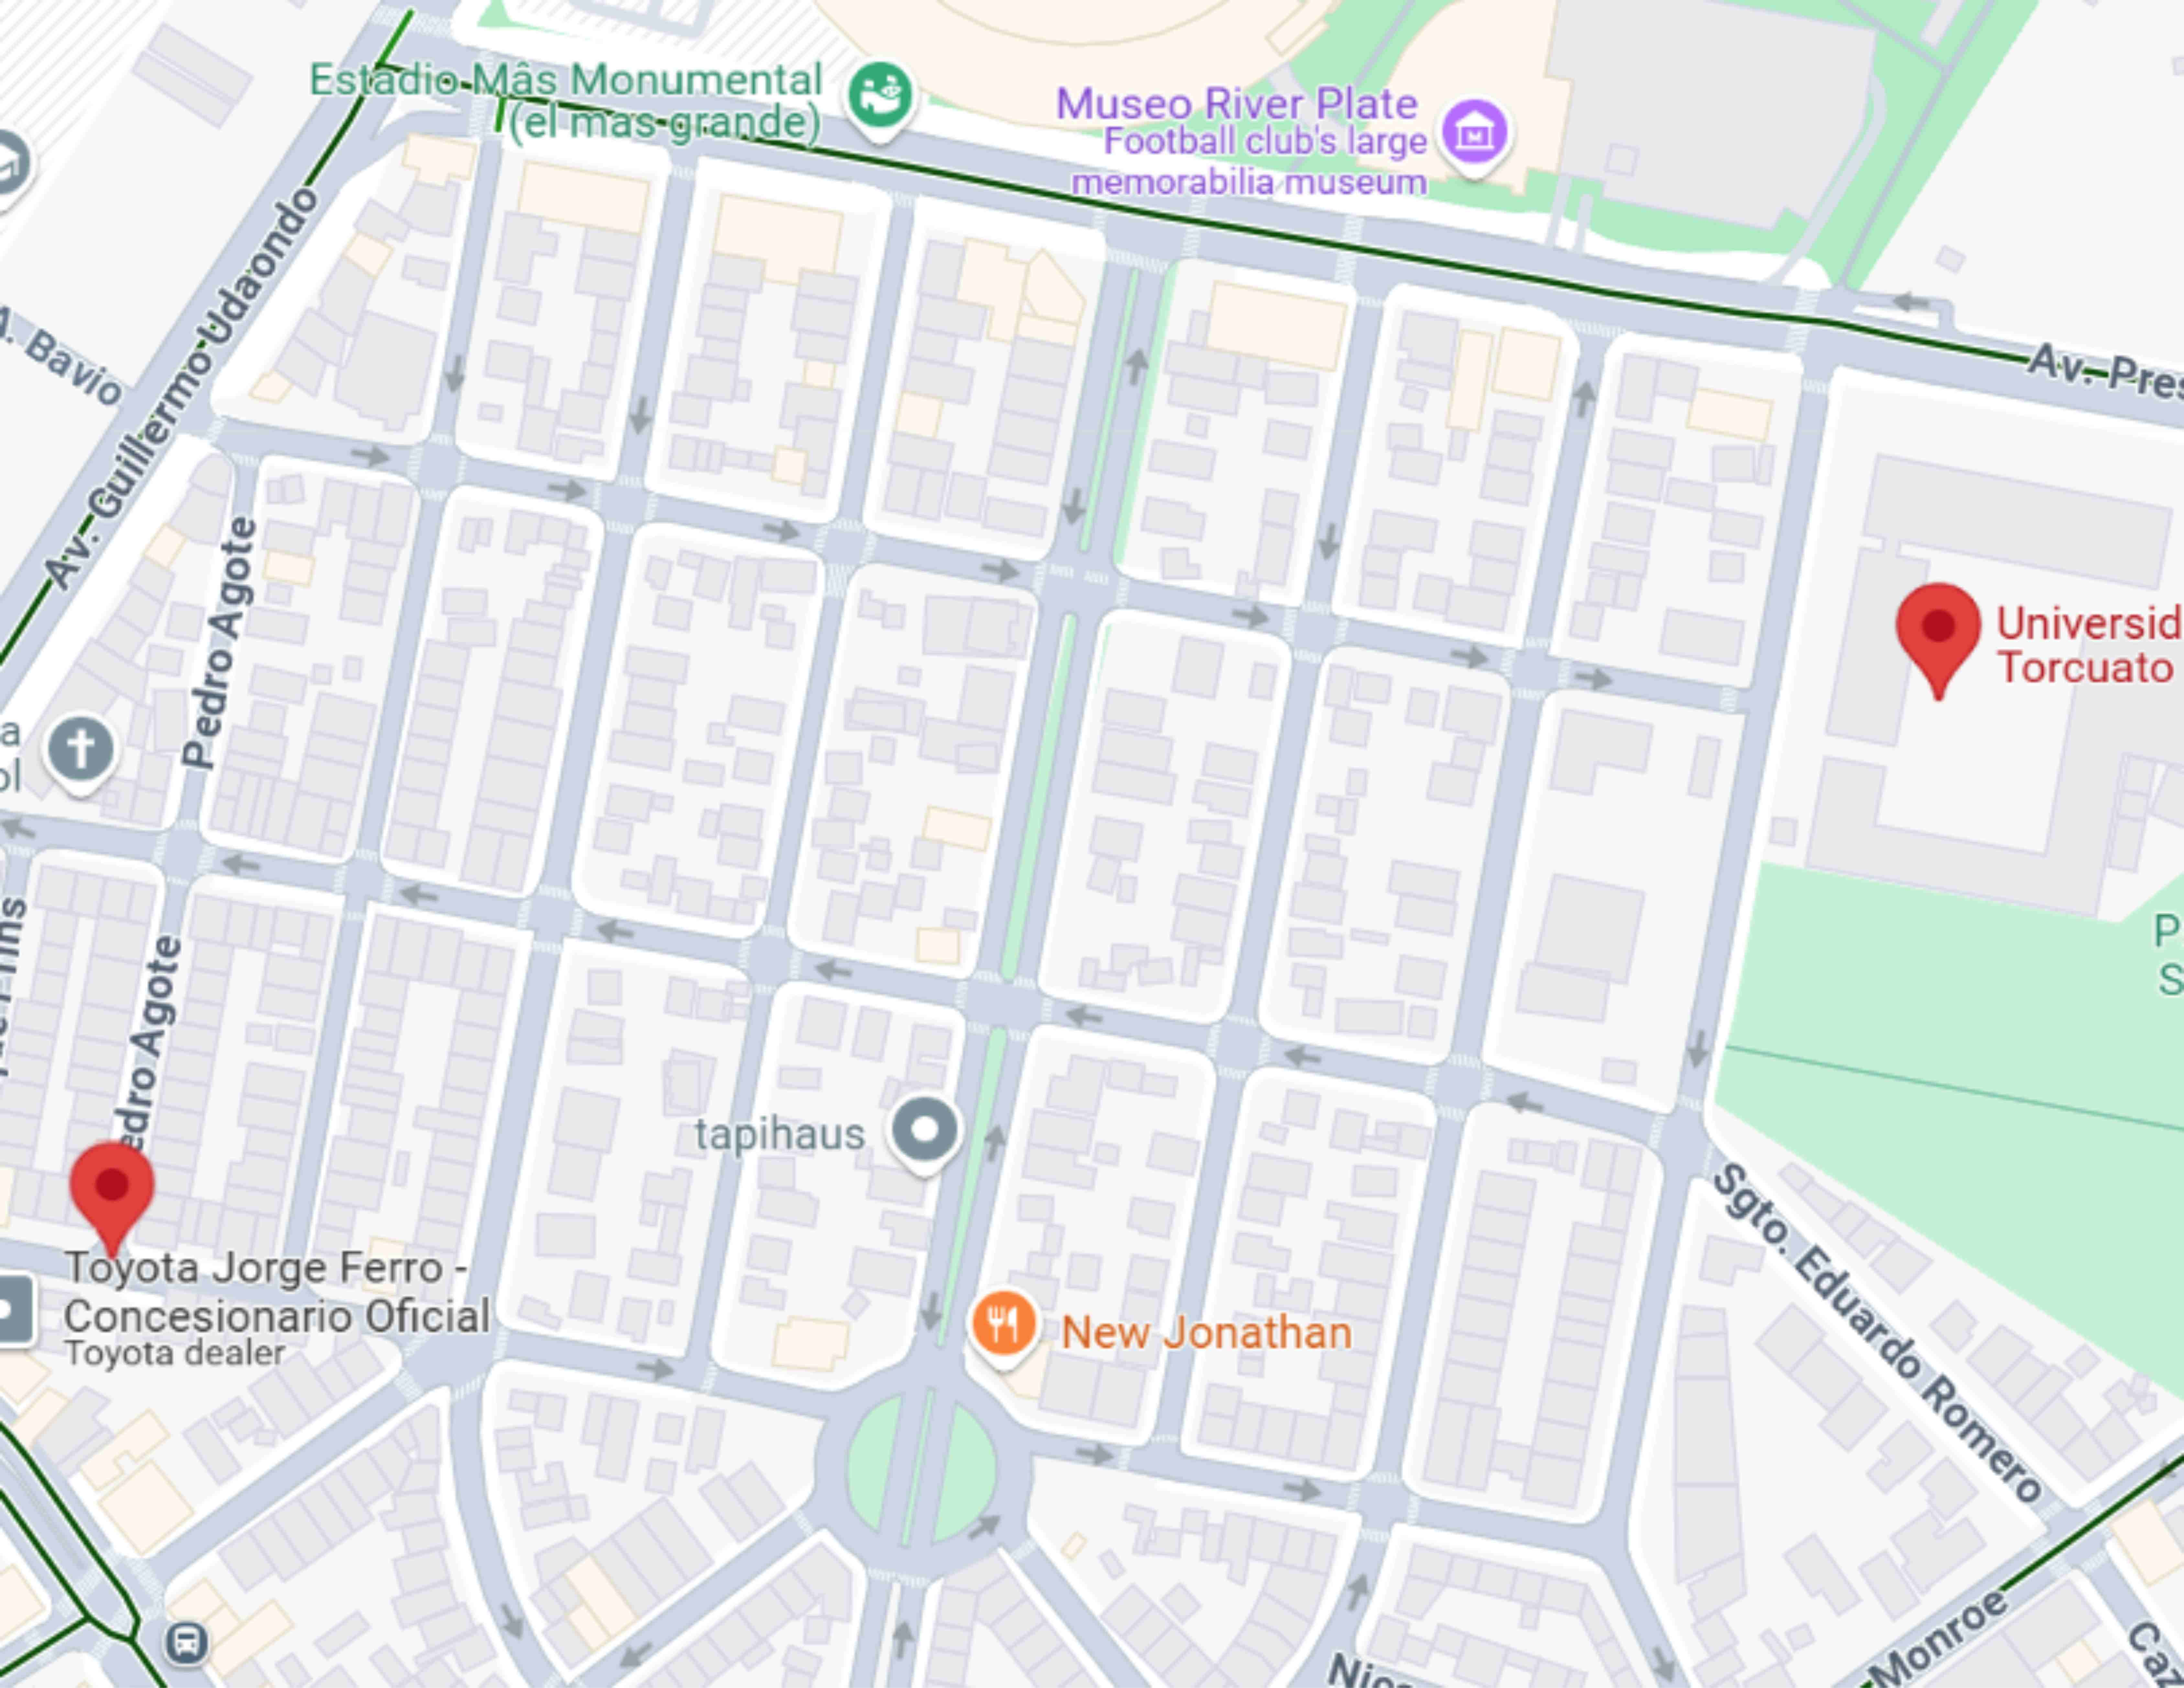
\includegraphics[width=0.8\textwidth]{../Images/Figures/mapa.jpg}
\end{center}
\end{frame}
\begin{frame}{Ejemplo: Ruta de Casa a La Universidad}
\begin{itemize}
\item Modelo MDP:
\begin{itemize}
\item<2-> Estado = posición en el mapa, en las esquinas
$x = (i,j)$
\item<3-> Acciones = desplazamiento, una cuadra por vez: 
$$
A = \left\{(0,1),(0,-1),(-1,0),(1,0)\right\} \equiv \left\{{\rm N}, {\rm S}, {\rm O}, {\rm E}\right\}
$$
\item<4-> Transición (determinística):
$$
x_{t+1} = \begin{cases}
x+a & {\rm if~}x_t \neq x^* \\
x^* & {\rm if~}x_t = x^*
\end{cases}
$$
\item<5-> Recompensa (castigo, en este caso):
$$
r_a(x) = 
\begin{cases} {\rm E}_w\left[tiempo(x,x+a,w)\right] & {\rm if}~ x \neq x^*\\
0 & {\rm if}~ x = x^*
\end{cases}
$$
\item<6-> Criterio de optimalidad:

\vspace{-0.5cm}
$$
\min_u {\rm E}\left[\sum\limits_{t=0}^\infty r_u(x_t)\right].
$$
\end{itemize}
\item<7-> Implementación en Python de Monte Carlo
\end{itemize}
\end{frame}
% --- SLIDE: BOOTSTRAPPING ---
\begin{frame}{Del Retorno al Bootstrapping}
\begin{itemize}
    \item \textbf{Limitaciones de Monte Carlo:}
    \begin{itemize}
        \item Solo se puede actualizar al \textbf{final} de la trayectoria (problema en episodios largos o infinitos).
        \item Alta varianza: cada retorno $R_t$ es la suma de muchas variables aleatorias.
    \end{itemize}
    
    \item<2-> \textbf{La Idea del Bootstrapping:} Relacionar el valor actual con el valor del estado siguiente.
    \[
    \begin{aligned}
    R_t &= r_t + \alpha \underbrace{(r_{t+1} + \alpha r_{t+2} + \dots)}_{R_{t+1}} \\
    &\approx r_t + \alpha \hat V(x_{t+1})
    \end{aligned}
    \]
    
    \item<3-> \textbf{Actualizaci\'on Incremental:} Podemos actualizar $\hat V(x_t)$ inmediatamente al observar la transici\'on $(x_t, r_t, x_{t+1})$:
    \[ \hat V(x_t) \leftarrow (1-\gamma_t)\hat V(x_t) + \gamma_t \underbrace{\left[ r_t + \alpha \hat V(x_{t+1}) \right]}_{\text{Target TD}} \]
\end{itemize}
\end{frame}

% --- SLIDE: TD-LEARNING ---
\begin{frame}{TD-Learning}
\begin{block}{Algoritmo TD(0)}
\begin{enumerate}
    \item Inicializar $\hat V(x)$ arbitrariamente (ej. ceros).
    \item Por cada paso en la experiencia $(x, r, x')$:
    \[ \hat V(x) \leftarrow \hat V(x) + \gamma \underbrace{\left[ \overbrace{r + \alpha \hat V(x')}^{\text{Target}} - \hat V(x) \right]}_{\text{Diferencia Temporal  (error de Bellman)}} \]
\end{enumerate}
\end{block}

\begin{itemize}
    \item<2-> \textbf{Visi\'on Te\'orica:} En cada iteraci\'on, se actualiza la funci\'on valor solo para el estado visitado  En promedio, la actualizaci\'on aproxima la direcci\'on de la ecuaci\'on de Bellman.
    \item<3-> \textbf{Ventaja Cr\'itica:} No necesitamos trayectorias completas. Podemos aprender de fragmentos sueltos de experiencia o de transiciones individuales de estado.
\end{itemize}
\end{frame}

% --- SLIDE: DE MRP A MDP ---
\begin{frame}{De la Evaluaci\'on a la Optimizaci\'on}
TD-Learning converge a $V_u$ para un proceso con política fija (MRP). ¿Podemos extender esto para encontrar la política óptima $V^*$?

\begin{itemize}
    \item<2-> \textbf{La Extensi\'on Natural:} En un MDP, el objetivo es satisfacer la ecuaci\'on de Bellman de optimalidad:
    \[ V^*(x) = \max_{a \in A} \mathbb{E} [r + \alpha V^*(y) \mid x, a] \]
    
    \item<3-> \textbf{TD para Optimalidad:} Si aplicamos la misma lógica de \textit{bootstrapping}, el "target" de nuestra actualización ahora incluye el operador de maximización:
    \[ \hat{V}(x) \leftarrow \hat{V}(x) + \gamma \left[ \max_{a \in A} (r_a + \alpha \hat{V}(y)) - \hat{V}(x) \right] \]
    
    \item<4-> \textbf{Garant\'ia Te\'orica:} Bajo condiciones de exploración suficientes, este esquema converge a la funci\'on valor óptima $V^*$.
\end{itemize}

\end{frame}

% --- SLIDE: EL OBSTÁCULO ---
\begin{frame}{Un Obst\'aculo en el Aprendizaje Directo}
\begin{itemize}
    \item TD-Learning nos permite obtener una estimativa de la la funci\'on valor $\hat{V}$. Con suficientes simulaciones, esa estimativa convergir\'a a $V^*$.
\end{itemize}

\begin{center}
\scalebox{0.85}{
\begin{tikzpicture}[
    node distance=5cm, 
    every node/.style={draw, thick, rounded corners, inner sep=8pt, font=\small, align=center},
    arrow/.style={-stealth, ultra thick}
]
  \node (data) [fill=gray!10] {Experiencias \\ $(x^i,a^i,r^i,y^i)$};
  \node (valor) [right of=data, fill=blue!5] {Estimaci\'on \\ de Valor $\hat V$};
  \node<4-> (politica) [right of=valor, fill=green!5] {Pol\'itica \\ Codiciosa $\hat u$};
  
  \draw<1-2> [arrow] (data) -- (valor);
  \draw<3> [arrow] (data) -- node[midway, above, font=\scriptsize, draw=none] {1. Aprender $V$} (valor);
 % \draw<4-> [arrow] (data) -- node[midway, above, font=\scriptsize, draw=none] {1} (valor);
  \draw<4-> [arrow] (valor) -- node[midway, above, font=\scriptsize, draw=none] {2. ¿C\'omo?} (politica);
\end{tikzpicture}}
\end{center}

\begin{itemize}
    \item<2-> \textbf{El Problema:} Para derivar la pol\'itica desde $\hat{V}$ necesitamos:
    \[ \hat u(x) = \arg\max_{a \in A} \left\{ \underbrace{r_a(x) + \alpha \sum_y P_a(x,y) \hat V(y)}_{\text{¡Requiere el Modelo!}} \right\} \]
    \item<3-> \textbf{Conclusi\'on:} Si no tenemos $P$ ni $r$, conocer $V^*$, mismo perfectamente, no es suficiente para actuar.
\end{itemize}
\end{frame}

% --- SLIDE: LA FUNCIÓN Q ---
\begin{frame}{La Soluci\'on: La Funci\'on $Q$}
La funci\'on $Q^*(x,a)$ representa el valor de tomar la acci\'on $a$ en el estado $x$ y seguir la pol\'itica \'optima de ah\'i en adelante.

\begin{itemize}
    \item \textbf{Definici\'on:} 
    \[ Q^*(x,a) = r_a(x) + \alpha \sum_y P_a(x,y) V^*(y) \]
    
    \item<2-> Como $V^*(x) = \max_a Q^*(x,a)$, podemos reescribir Bellman:
    \[ Q^*(x,a) = r_a(x) + \alpha \sum_y P_a(x,y) \max_{a' \in A} Q^*(y,a') \]
    
    \item<3->  Con una aproximaci\'on $\hat Q$, la pol\'itica es \textbf{directa}:
    \[ \hat u(x) = \arg\max_{a \in A} \hat Q(x,a) \]
    \textit{¡No necesitamos conocer las probabilidades de transici\'on $P$!}
\end{itemize}
\end{frame}

% --- SLIDE: Q-LEARNING ALGORITMO ---
\begin{frame}{Algoritmo: Q-Learning}
\begin{block}{Q-Learning (Watkins, 1989)}
\begin{enumerate}
    \item Inicializar $\hat Q(x,a)$ arbitrariamente.
    \item Por cada transici\'on observada $(x, a, r, y)$:
    \[ \hat Q(x,a) \leftarrow \hat Q(x,a) + \gamma \underbrace{\left[ \overbrace{r + \alpha \max_{a' \in A} \hat Q(y,a')}^{\text{Target (Bellman)}} - \hat Q(x,a) \right]}_{\text{Diferencia Temporal (TD)}} \]
    \item Repetir hasta convergencia.
\end{enumerate}
\end{block}

\begin{itemize}
    \item<2-> \textbf{Intuici\'on:} Si el término entre corchetes es positivo, la acción $a$ resultó ser mejor de lo que esperábamos $\rightarrow$ aumentamos $\hat Q(x,a)$.
    \item<3-> \textbf{Off-policy:} Podemos aprender de \textbf{cualquier} dato (incluso si la acción $a$ fue tomada por una política mediocre o al azar).
\end{itemize}
\end{frame}

% --- SLIDE: CALIBRACIÓN DE PARÁMETROS ---
\begin{frame}{Calibraci\'on y Desaf\'ios Pr\'acticos}
La implementaci\'on exitosa de Q-Learning exige una sinton\'ia fina. No basta con programar la f\'ormula; hay que gestionar c\'omo aprende el agente.

\begin{itemize}
    \item \textbf{Tasa de Aprendizaje ($\gamma$):} 
    Controla el balance entre la \textbf{memoria} (lo aprendido) y la \textbf{novedad} (la muestra actual). Determina la estabilidad frente al ruido.
    
    \item \textbf{Exploraci\'on vs. Explotaci\'on}
    ¿Qu\'e acciones debemos elegir? ¿Usamos lo que ya funciona o buscamos algo mejor?
    
    \item \textbf{Desaf\'ios de Ingenier\'ia:} 
    Incluso con par\'ametros óptimos, enfrentaremos problemas de sesgo, correlaci\'on y escasez de recompensas.
\end{itemize}

\end{frame}
% --- SLIDE 1: EL DILEMA ---
\begin{frame}{Exploraci\'on vs Explotaci\'on}
Para que $\hat Q \to Q^*$, el agente debe \textbf{explorar suficientemente} el espacio de acciones. 

\begin{itemize}

\item En principio, podemos tomar acciones aleatorias, en estados aleatorios, y la convergencia est\'a garantizada.

    \item<2-> \textbf{Eficiencia:} El azar puro garantiza convergencia, pero es computacionalmente lento.
    
    \item<3-> \textbf{Online Learning (En Vivo):}
    Dilema econ\'omico: explorar es costoso (p\'erdida de recompensa real).

\end{itemize}

\visible<4->{
\begin{block}{La Pol\'itica $\epsilon$-greedy}
Equilibrio base entre búsqueda y aprovechamiento:
\[
a_t = \begin{cases} 
\arg\max_{a} Q(x,a) & \text{con prob. } 1-\epsilon \ (\text{Explotaci\'on}) \\
\text{acci\'on aleatoria} & \text{con prob. } \epsilon \ (\text{Exploraci\'on})
\end{cases}
\]
\end{block}}
\end{frame}

% --- SLIDE 2: MÁS ALLÁ DE EPSILON-GREEDY ---
\begin{frame}{Estrategias Avanzadas de Exploraci\'on}
$\epsilon$-greedy explora a ciegas. Alternativas para problemas complejos:

\begin{itemize}
    \item \textbf{Exploraci\'on de Boltzmann (Softmax):}
    Selecci\'on probabil\'istica seg\'un el valor estimado:
    \[ P(a|x) \propto e^{Q(x,a)/\tau} \]
    Evita acciones desastrosas al priorizar opciones casi-\'optimas.

    \item \textbf{Optimismo (UCB / Initial Values):}
    Inicializar $Q$ con valores muy altos. Fuerza la exploraci\'on inicial hasta que la realidad corrige las expectativas.

    \item \textbf{Seguro contra el cambio:}
    En entornos \textbf{no estacionarios}, mantener $\epsilon > 0$ permite detectar cambios estructurales en el sistema.
\end{itemize}
\end{frame}


% --- SLIDE: TASA DE APRENDIZAJE (ACTUALIZADA) ---
\begin{frame}{Tasa de Aprendizaje: Memoria vs. Ruido}
Podemos reescribir la actualizaci\'on de Q-Learning para ver c\'omo $\gamma$ pondera la informaci\'on. Por cada transici\'on observada $(x, a, r, y)$:
\[ 
\underbrace{\hat Q(x,a)}_{\text{Nuevo Valor}} \leftarrow (1-\gamma) \underbrace{\hat Q(x,a)}_{\text{Valor Anterior}} + \gamma \underbrace{\left[ r + \alpha \max_{a' \in A} \hat Q(y,a') \right]}_{\text{Nueva Muestra (Target)}} 
\]

\begin{itemize}
    \item <2->\textbf{$\gamma$ alto (ej: 0.5):} 
    \begin{itemize}
        \item \textit{Ventaja:} El algoritmo incorpora informaci\'on nueva r\'apidamente.
        \item \textit{Riesgo:} Alta \textbf{varianza}. Si las muestras son ruidosas, $Q$ oscilar\'a sin converger.
    \end{itemize}
    \item<3-> \textbf{$\gamma$ bajo (ej: 0.01):} 
    \begin{itemize}
        \item \textit{Ventaja:} Estable ante el ruido; act\'ua como un filtro de media m\'ovil.
        \item \textit{Riesgo:} Aprendizaje muy lento (\textit{estancamiento}).
    \end{itemize}
\end{itemize}

\visible<4->{
\begin{alertblock}{En la pr\'actica}
    Si el entorno es \textbf{no estacionario} (cambiante), nunca debemos llevar $\gamma$ a cero, o el agente dejar\'a de notar los cambios en el sistema.
\end{alertblock}}
\end{frame}

% --- SLIDE: INTRODUCCIÓN TEMAS AVANZADOS ---
\begin{frame}{[Temas Avanzados] Desaf\'ios en la Pr\'actica}
Aplicar Q-Learning tabular a problemas reales suele fallar por tres motivos:
\begin{enumerate}
    \item \textbf{Escasez de Se\~nal:} El agente no encuentra recompensas (sparse rewards).
    \item \textbf{Inestabilidad:} Los datos est\'an correlacionados temporalmente.
    \item \textbf{Sobreestimaci\'on:} El ruido hace que el agente sea "demasiado optimista".
\end{enumerate}

\end{frame}

% --- SLIDE: TEMAS AVANZADOS: REWARD SHAPING ---
\begin{frame}{[Temas Avanzados] Reward Shaping}
\begin{itemize}
    \item \textbf{Problema:} En algunas tareas, el agente recibe $0$ casi siempre. \textquestiondown Examples?
    \item<2-> \textbf{Soluci\'on:} Dise\~nar recompensas intermedias para guiar el aprendizaje.
    \item<3-> \textbf{Peligro:} \textit{Reward Hacking}. El agente puede encontrar un atajo para ganar puntos sin resolver la tarea (ej: un robot que da vueltas en c\'irculos para ganar "puntos por movimiento").
\end{itemize}
\end{frame}

% --- SLIDE 3: [AVANZADO] DOUBLE Q-LEARNING ---
\begin{frame}{[Temas Avanzados] Double Q-Learning: Sesgo y Jensen}
\textbf{El Problema:} El operador $\max$ es convexo. Por la \textbf{Desigualdad de Jensen}, el ruido inyecta un sesgo de sobreestimaci\'on:
\[ \mathbb{E}[\max_{a} \hat{Q}(s, a)] \geq \max_{a} \mathbb{E}[\hat{Q}(s, a)] \]

\begin{itemize}
    \item \textbf{Soluci\'on:} Desacoplar \textbf{selecci\'on} de \textbf{evaluaci\'on}.
    \item \textbf{Mec\'anica (Sim\'etrica):} Mantener $Q_1$ y $Q_2$. \textbf{Actualizar $Q_1$ o $Q_2$, aleatoriamente.} Si actualizamos $Q_1$:
    \begin{enumerate}
        \item \textbf{Selecci\'on:} $a^* = \arg\max_{a} Q_1(y, a)$ 
        \item \textbf{Evaluaci\'on:} El target se calcula con la \textit{otra} tabla:
        \[ Q_1 \leftarrow Q_1 + \gamma [ r + \alpha Q_2(y, a^*) - Q_1 ] \]
    \end{enumerate}
\end{itemize}

\begin{exampleblock}{Intuici\'on de Ensamble}
    La ">segunda opini\'on"< de un estimador independiente elimina el optimismo sistem\'atico del ruido.
\end{exampleblock}
\end{frame}

% --- SLIDE: TEMAS AVANZADOS: EXPERIENCE REPLAY ---
\begin{frame}{[Temas Avanzados] Experience Replay}
\begin{itemize}
    \item \textbf{Problema:} Los datos $(x, a, r, y)$ en una trayectoria est\'an altamente correlacionados. Esto hace que el aprendizaje sea inestable.
    \item \textbf{Soluci\'on:} Guardar las experiencias en un \textit{buffer} (memoria) y entrenar extrayendo mini-batches al azar.
    \item \textbf{Beneficio:} Rompe la correlaci\'on temporal y permite aprender varias veces de experiencias valiosas.
\end{itemize}
\end{frame}

% --- SLIDE: CONCLUSIONES ---
\begin{frame}{Conclusiones: De la Teor\'ia a la Implementaci\'on}
El paso de la programaci\'on din\'amica al aprendizaje por refuerzo implica gestionar la incertidumbre y el ruido.

\begin{itemize}
    \item \textbf{El poder del Bootstrapping:} TD-Learning permite aprender sin un modelo del entorno, actualizando estimaciones basadas en otras estimaciones.
    
    \item \textbf{Calibraci\'on como Prioridad:} El exito no depende solo del algoritmo, sino del equilibrio entre \textbf{exploraci\'on} (cobertura) y \textbf{tasa de aprendizaje} (estabilidad vs. velocidad).


    \item \textbf{Pensamiento de Diseño:} Como cient\'ificos, nuestro rol es dise\~nar incentivos (recompensas) y estructuras que permitan que la raz\'on sirva a la existencia del agente en entornos complejos.
\end{itemize}

\end{frame}

% --- SLIDE 2: REVISIÓN AGENTE/AMBIENTE ---
\begin{frame}{Revisi\'on - MDPs y Aprendizaje por Refuerzo}
\begin{center}
\includegraphics[width=0.5\textwidth]{../Images/Figures/LearningCycle3.jpg}
\end{center}
\vspace{-2.5cm}
\begin{columns}[t]
\hspace{1.0cm}\begin{column}{0.5\textwidth}
\begin{itemize}
    \item<3-> \textbf{Agente:}
    \begin{itemize}
    \item Funci\'on valor $V(x)$ o $Q(x,a)$
    \item Pol\'itica $u(x)$
    \end{itemize}
\end{itemize}
\end{column}
\begin{column}{0.5\textwidth}
\begin{itemize}
    \item<2-> \textbf{Ambiente:} 
    \begin{itemize}
    \item Recompensa $r_a(x)$
    \item Transici\'on $P_a(x,y)$
    \end{itemize}
\end{itemize}   
\end{column}
\end{columns}
\end{frame}

% --- SLIDE 3: REVISIÓN BELLMAN ---
\begin{frame}{Revisi\'on - Ecuaci\'on de Bellman}
\begin{itemize}
\item La funci\'on valor \'optima satisface:
$$
\begin{array}{ccl}
V^*(x) & = &  \max\limits_{a \in A}\left\{r_a(x) + \alpha \sum_y P_a(x,y)V^*(y)\right\} \\
Q^*(x,a) & = & r_a(x) + \alpha \sum_y P_a(x,y)\max\limits_{a' \in A} Q^*(y,a')
\end{array}
$$
\item<2-> Estrategias de soluci\'on:
\begin{center}
\small
\begin{tabular}{|l|l|}
  \hline
  \textbf{Soluciones Exactas} & \textbf{Aprendizaje (Model-Free)} \\
  \hline
  Iteraci\'on de valor & Monte Carlo (Pol\'itica fija) \\
  Iteraci\'on de pol\'itica & TD-Learning / \textbf{Q-Learning} \\
  \hline
\end{tabular}
\end{center}
\item<3-> En ambos casos, el objetivo es derivar la pol\'itica \'optima $u^*(x)$. 
\end{itemize}
\end{frame}

% --- SLIDE 4: Q-LEARNING (REPASO) ---
\begin{frame}{Revisi\'on - Q-Learning Tabular}
\begin{block}{Algoritmo}
\begin{enumerate}
\item Inicializar tabla $\hat Q$ y $t=1$.
\item Seleccionar acci\'on $a^i$ (ej: $\epsilon$-greedy).
\item Observar $(x^i, a^i, r^i, y^i)$ y actualizar:
{\small
\[ \hat Q(x^i,a^i) \leftarrow \hat Q(x^i,a^i) + \gamma_i \left[ r^i + \alpha \max_{a} \hat Q(y^i, a) - \hat Q(x^i, a^i) \right] \]
}
\item Hacer $t = t+1$ y volver al paso 2.
\end{enumerate}  
\end{block}
\begin{itemize}
\item<2-> \textbf{Learning rate ($\gamma_i$):} Controla la convergencia. Ej: $\gamma_i = 1/N(x,a)$.
\item<3-> \textbf{Limitaci\'on fundamental:} Cada par $(x,a)$ es una celda independiente en la tabla.
\end{itemize}
\end{frame}

% --- SLIDE 5: DIMENSIONALIDAD (MAPA) ---
\begin{frame}{La “Maldici\'on de la Dimensionalidad”}
\begin{itemize}
\item El enfoque tabular requiere almacenar $V^*$ o $Q^*$ en memoria.
\item<2-> Imaginemos una tienda que debe decidir cu\'anto pedir de cada producto para minimizar costos de almacenamiento y faltantes. \textquestiondown C\'omo modelamos el estado?

\begin{itemize}
    \item<3-> \textbf{Estado:} Nivel de stock de cada producto.
    \item<4-> \textbf{1 Producto:} Si la capacidad es de 100 unidades $\rightarrow$ \textbf{100 estados}. (F\'acil)
    \item<5-> \textbf{3 Productos:} $100 \times 100 \times 100 = 10^6$ $\rightarrow$ \textbf{1 mill\'on de estados}. (Al l\'imite de una tabla)
    \item<6-> \textbf{10 Productos:} $100^{10} = 10^{20}$ estados. 
\end{itemize}
\end{itemize}

\begin{alertblock}{El Problema de la Realidad}
    Hay m\'as estados en este inventario de 10 productos que granos de arena en la Tierra ($\approx 10^{19}$). \textbf{Es imposible llenar esta tabla}, incluso con toda la capacidad de cómputo actual.
\end{alertblock}
\end{frame}

% --- SLIDE: EJEMPLO GO (REGLAS) ---
\begin{frame}{Ejemplo: Go}
\begin{center}
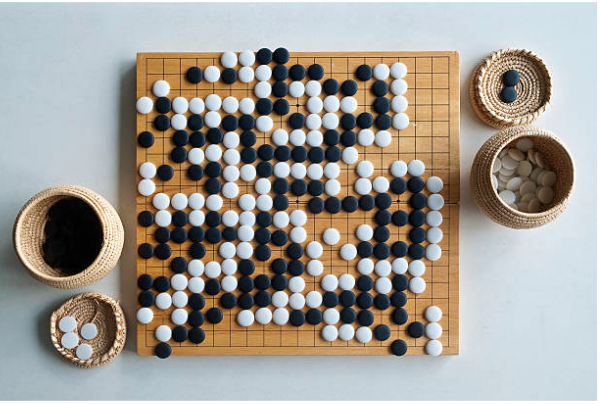
\includegraphics[width=0.8\textwidth]{../Images/Figures/Go1.png}
\end{center}
\end{frame}

% --- SLIDE: EJEMPLO GO (ALPHAGO) ---
\begin{frame}{Ejemplo: Go (La Evoluci\'on)}
\begin{center}
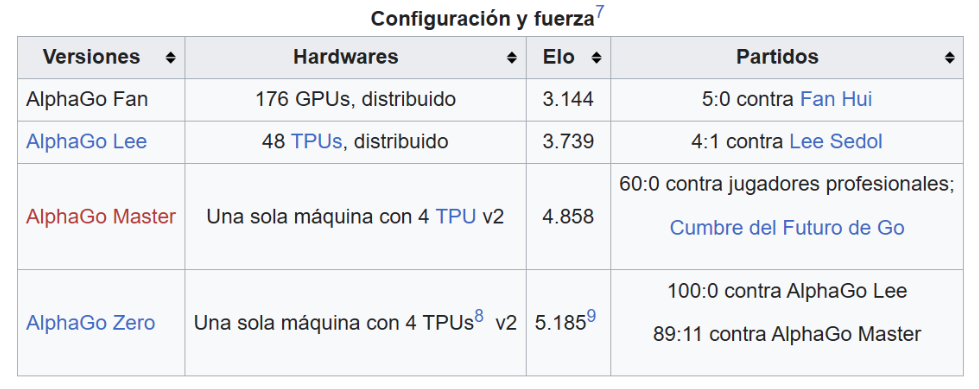
\includegraphics[width=1\textwidth]{../Images/Figures/Go2.png}
\end{center}    
\end{frame}

% --- SLIDE: EJEMPLO GO - ¿CUÁNTOS ESTADOS? ---
\begin{frame}{Ejemplo: Go - ¿Cu\'antos estados?}
\begin{itemize}
\item Tablero de $19\times19$
\begin{itemize} 
\item $19 \times 19 = 361$ variables de estado (posiciones).
\item Cada posici\'on tiene 3 valores: \{blanco, negro, vac\'io\}.
\item \textbf{Crecimiento Exponencial:} $3^{361}$ combinaciones totales. 
\end{itemize}

\item<2-> Determinar cu\'antas de esas configuraciones son \textit{v\'alidas} seg\'un las reglas del Go es, en s\'i mismo, un problema masivo.
\begin{itemize}
    \item<3-> En 2015, John Tromp requiri\'o \textbf{9 meses de procesamiento} en computadores de alta potencia para hallar el n\'umero exacto:

$208168199381979984699478633344862770286522453884$

$530548425639456820927419612738015378525648451698$

$519643907259916015628128546089888314427129715319$

$317557736620397247064859013377169378226061371114$

$670302056198056 \approx \mathbf{2 \times 10^{170}}$ \textbf{configuraciones v\'alidas}
\end{itemize}
\end{itemize}


\begin{alertblock}{Conclusi\'on}<4->
    Si solo \textbf{contar} los estados toma meses de superc\'omputo, una tabla de Q-Learning es f\'isicamente inviable. 
\end{alertblock}
\end{frame}

% --- SLIDE 1: EL PROBLEMA — LA MALDICIÓN DE LA DIMENSIONALIDAD ---
\begin{frame}{La “Maldici\'on de la Dimensionalidad”}
\begin{itemize}
    \item  El n\'umero de estados crece \textbf{exponencialmente} respecto al n\'umero de variables de estado.
    \item En problemas reales (Go, Inventarios, Finanzas), el espacio de b\'usqueda es tan vasto que no se puede visitar, calcular ni almacenar.
\end{itemize}

\visible<2->{
\begin{exampleblock}{Ejemplo: Control de Inventarios (10 productos)}
    Si cada producto tiene 100 niveles de stock:
    \begin{itemize}
        \item Estados posibles: $100^{10} = 10^{20}$.
        \item \textbf{El error de la tabla:} Trata 99 unidades como algo totalmente distinto a 100 unidades. No hay transferencia de conocimiento.
    \end{itemize}
\end{exampleblock}}

\visible<3-> {\begin{center}\textbf{Si el espacio de estados es prohibitivo, la memoria debe ser reemplazada por la generalizaci\'on.}\end{center}}
\end{frame}

% --- SLIDE 2: LA SOLUCIÓN — APROXIMACIÓN Y GENERALIZACIÓN ---
\begin{frame}{De la Memoria a la Generalizaci\'on}
\begin{itemize}
    \item \textbf{Soluci\'on:} Sustituir la tabla por una \textbf{forma param\'etrica} $f(x, \theta)$.
    \item \textbf{Aproximaci\'on de Funciones:} 
    Pasamos de estimar $10^{20}$ celdas a estimar un vector de pesos $\theta \in \Re^K$ (donde $K \ll$ estados).
    \[ V^*(x) \approx f(x,\theta_V) \quad ; \quad Q^*(x,a) \approx f(x, a, \theta_Q) \]
    
    \item<2-> \textbf{Generalizaci\'on (Ventaja Cr\'itica):} 
    Al aprender sobre un estado visitado, el modelo "entiende" la tendencia para estados similares no visitados.
\end{itemize}

\only<3->{
\begin{block}{Cambio de Paradigma}
    Ya no buscamos el valor exacto de cada casilla, sino los \textbf{pesos} $\theta$ que mejor describen la \textbf{estructura} de la funci\'on de valor $V$ o $Q$.
\end{block}}

%\begin{itemize}
%    \item<4-> \textit{Nota:} Tambi\'en podemos parametrizar la pol\'itica $u(x,a,\theta_u)$ como una distribuci\'on de probabilidad.
%\end{itemize}
\end{frame}



\begin{frame}{Aproximaciones Lineales}
\begin{itemize}
\item Queremos aproximar el valor de un estado \( V(x) \) sin usar una tabla
\item<2-> Usamos una combinación de funciones conocidas ("funciones básicas"):
\begin{center}
\begin{tikzpicture}[
  node distance=1.2cm and 1.5cm,
  every node/.style={font=\small},
  input/.style={draw, rectangle, minimum width=1.5cm, minimum height=0.8cm, fill=gray!10, rounded corners},
  func/.style={draw, circle, minimum size=1.1cm, fill=white},
  output/.style={draw, rectangle, minimum width=2.5cm, minimum height=0.9cm,  fill=gray!10, rounded corners},
  weight/.style={font=\footnotesize, blue!80!black}
]

% Nodes
\node[input] (state) {Estado $x$};

\node[func, right=of state, yshift=1.5cm] (f1) {$\phi_1(x)$};
\node[func, right=of state]               (f2) {$\phi_2(x)$};
\node[func, right=of state, yshift=-1.5cm] (fk) {$\phi_K(x)$};

\node[output, right=of f2] (value) {Valor $\hat{V}(x, \theta) = \sum_{i=1}^K \theta_i \phi_i(x)$};

% Lines from state to features
\draw[->] (state.east) -- (f1.west);
\draw[->] (state.east) -- (f2.west);
\draw[->] (state.east) -- (fk.west);

% Lines from features to value
\draw[->] (f1.east) -- (value.west) node[midway, above, weight] {$\theta_1$};
\draw[->] (f2.east) -- (value.west) node[midway, above, weight] {$\theta_2$};
\draw[->] (fk.east) -- (value.west) node[midway, above, weight] {$\theta_K$};

% Main Formula
%\node[above=0.2cm of value] {\small $\hat{V}(x, \theta) = \sum_{i=1}^K \theta_i \phi_i(x)$};
\end{tikzpicture}
\end{center}
\item<3-> La aproximaci\'on es  \textbf{lineal en los parámetros $\mathbf{\theta}$} (aunque \( \phi_i(x) \) normalmente son no lineales en $x$)
\end{itemize}
\end{frame}


% --- SLIDE 1: APROXIMACIÓN LINEAL ---
\begin{frame}{Aproximaciones Lineales: Ejemplos}

\begin{center}
\begin{tikzpicture}[
  node distance=1.2cm and 1.5cm,
  every node/.style={font=\small},
  input/.style={draw, rectangle, minimum width=1.5cm, minimum height=0.8cm, fill=gray!10, rounded corners},
  func/.style={draw, circle, minimum size=1.1cm, fill=white},
  output/.style={draw, rectangle, minimum width=2.5cm, minimum height=0.9cm,  fill=gray!10, rounded corners},
  weight/.style={font=\footnotesize, blue!80!black}
]

% Nodes
\node[input] (state) {Estado $x$};

\node[func, right=of state, yshift=1.5cm] (f1) {$\phi_1(x)$};
\node[func, right=of state]               (f2) {$\phi_2(x)$};
\node[func, right=of state, yshift=-1.5cm] (fk) {$\phi_K(x)$};

\node[output, right=of f2] (value) {Valor $\hat{V}(x, \theta) = \sum_{i=1}^K \theta_i \phi_i(x)$};

% Lines from state to features
\draw[->] (state.east) -- (f1.west);
\draw[->] (state.east) -- (f2.west);
\draw[->] (state.east) -- (fk.west);

% Lines from features to value
\draw[->] (f1.east) -- (value.west) node[midway, above, weight] {$\theta_1$};
\draw[->] (f2.east) -- (value.west) node[midway, above, weight] {$\theta_2$};
\draw[->] (fk.east) -- (value.west) node[midway, above, weight] {$\theta_K$};

% Main Formula
%\node[above=0.2cm of value] {\small $\hat{V}(x, \theta) = \sum_{i=1}^K \theta_i \phi_i(x)$};
\end{tikzpicture}
\end{center}
\begin{itemize}
  \item<2-> \textbf{Estado directo:} $\phi_i(x) = x_i$.
  \item<3-> \textbf{Polinomios:} Combinaciones como $x_1^2, x_1 x_2 \dots$ para capturar relaciones.
  \item<4-> \textbf{Otras Funciones Base:} Uso de $\sin(x), \log(x)$ o RBFs para mayor flexibilidad.
  \item<5-> \textbf{Agregaci\'on de estados:} Dividir el espacio en regiones disjuntas.
\end{itemize}
\end{frame}

% --- SLIDE 2: AGREGACIÓN DE ESTADOS ---
\begin{frame}{Agregaci\'on de Estados}
\[
\phi_i(x) = \begin{cases}
1 & \text{si } x \in S_i \\
0 & \text{si } x \notin S_i
\end{cases}
\]   
\begin{columns}[T]
\begin{column}{0.5\textwidth}
\begin{itemize}
\item<2-> \textbf{Idea:} Agrupar estados similares en zonas.
\item<3-> El valor aproximado es constante dentro de cada zona: $\hat{V}(x) = \theta_i$.
\item<4-> \textbf{Ventaja:} Simplifica el problema y garantiza estabilidad.
\item<5-> \textbf{Desaf\'io:} Requiere una buena partici\'on del espacio para no perder detalles cr\'iticos.
\end{itemize}
\end{column}
\begin{column}{0.5\textwidth}
\begin{center}
\visible<2->{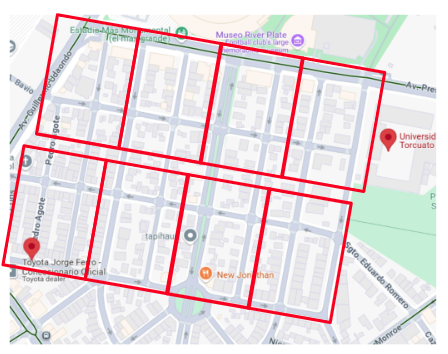
\includegraphics[width=0.9\textwidth]{../Images/Figures/StateAggregation.png}}
\end{center}
\end{column}
\end{columns}
\end{frame}

% --- SLIDE 3: APROXIMACIÓN NO LINEAL ---
\begin{frame}{Aproximaciones No Lineales}
\[
\hat{V}(x, \theta) \approx f(x, \theta)
\]
\begin{itemize}
\item La funci\'on $f$ es \textbf{no lineal} respecto a los par\'ametros $\theta$.
\item<2-> \textbf{Ejemplo principal:} Redes Neuronales Artificiales.
\item<3-> Permite extraer caracter\'isticas autom\'aticamente de datos ">crudos"< (im\'agenes, audio).
\item<4-> Es la base del \textbf{Deep Reinforcement Learning}.
\end{itemize}

\begin{center}
\visible<2->{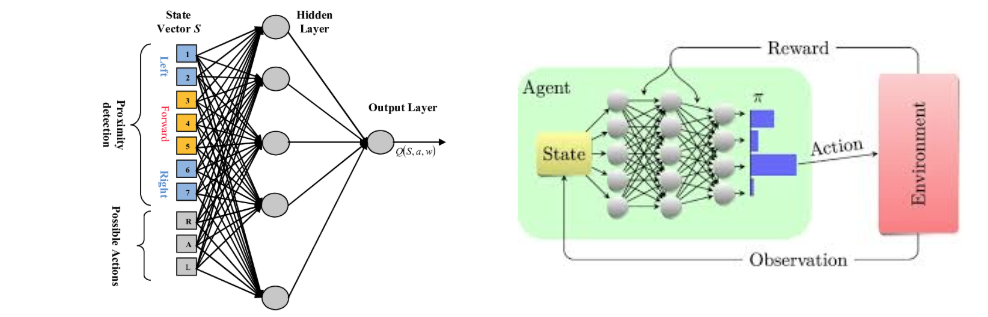
\includegraphics[width=0.7\textwidth]{../Images/Figures/NeuralNetwork.png}}
\end{center}
\end{frame}

% --- SLIDE 1: ARQUITECTURAS Y EXPRESIONES ---
\begin{frame}{Arquitecturas de Aproximaci\'on}
\centering

% Iniciamos un grupo para que el tamaño reducido solo afecte a la tabla
{\tiny
\setlength{\tabcolsep}{2pt}
\begin{tabular}{|l|c|c|c|c|}
\hline
\textbf{Categor\'ia} & \textbf{Agregaci\'on} & \textbf{Lineal en $\theta$ (Manual)} & \textbf{No Lineal en $\theta$ (Manual)} & \textbf{No Lineal en $\theta$ (Universal)} \\ \hline
\rule{0pt}{4ex} \textbf{Expresi\'on} & $\displaystyle \sum \theta_i \mathbb{I}_i(x)$ & $\displaystyle \sum \theta_i \phi_i(x)$ & $\displaystyle f_{expert}(x, \theta)$ & $\displaystyle f_{NN}(x, \theta)$ \\ [2ex] \hline
\textbf{Representaci\'on} & Zonas fijas & Features $\phi(x)$ fijas & Estructura fijada por experto & Features aprendidas \\ \hline
\textbf{Dependencia $\theta$} & Lineal & Lineal & No Lineal & No Lineal \\ \hline
\textbf{Ejemplos} & Grillas / Tiles & Polinomios, Fourier & Modelos f\'isicos, Sigmoides & Redes Neuronales \\ \hline
\end{tabular}
} % Aquí termina el efecto de \tiny

\vspace{0.5cm}

% Este bloque ahora tendrá el tamaño de letra estándar de la presentación
\begin{alertblock}{Dependencia de Par\'ametros}
    La distinci\'on \textbf{Lineal / No Lineal} define si el valor es una combinaci\'on lineal de los par\'ametros $\theta$, independientemente de $x$.
    \begin{itemize}
  \item Un modelo No Lineal Manual inyecta estructura experta donde $\theta$ no act\'ua como un simple peso.
    \end{itemize}
\end{alertblock}
\end{frame}

% --- SLIDE 2: COMPARATIVA TÉCNICA ---
\begin{frame}{Comparativa de Convergencia}
\small
\begin{itemize}
    \item \textbf{Agregaci\'on de Estados:}
    \begin{itemize}
        \item Recupera \textbf{garant\'ias de convergencia} del caso tabular.
        \item Representaci\'on r\'igida (escalonada).
    \end{itemize}
    
    \item \textbf{Dise\~no de Features (Lineal en $\theta$):}
    \begin{itemize}
        \item Superficie de error cuadr\'atica respecto a targets fijos.
        \item El experto gu\'ia" al modelo mediante $\phi(x)$.
    \end{itemize}

    \item \textbf{Modelos Estructurales (No Lineal Manual):}
    \begin{itemize}
        \item Inyecta leyes f\'isicas o l\'imites estructurales.
        \item \textbf{No convexo:} Dif\'icil de optimizar pese a pocos par\'ametros.
    \end{itemize}

    \item \textbf{Aproximadores Universales (Redes):}
    \begin{itemize}
        \item La red extrae sus propias features (\textit{Representation Learning}).
        \item M\'axima flexibilidad; mayor riesgo de inestabilidad.
    \end{itemize}
\end{itemize}

\begin{block}{Criterio de Selecci\'on}
    \textbf{Manual:} Si conoces la forma funcional de la relaci\'on. \\
    \textbf{Universal:} Si el problema es una caja negra compleja.
\end{block}
\end{frame}

\begin{frame}{RL con Aproximaci\'on}
\begin{columns}[T]
\begin{column}{0.42\textwidth}
    \centering
    \begin{tikzpicture}[scale=0.85]
        % Ejes
        \draw[->] (0,0) -- (4,0) node[right] {\tiny $x$};
        \draw[->] (0,0) -- (0,2.5) node[above] {\tiny $V(x)$};
        
        % Muestras (ruidosas)
        \foreach \p in {(0.5,0.6), (0.8,1.2), (1.2,0.9), (1.5,1.8), (2.0,1.5), (2.5,2.4), (3.0,2.1)}
            \fill[red!70!black] \p circle (1.2pt);
            
        % Curva paramétrica
        \draw[blue, thick] plot [smooth, tension=0.6] coordinates {(0,0.4) (1,1.1) (2,1.7) (3,2.3) (4,2.5)};
        
        % Leyenda
%        \node[red!70!black, font=\tiny, anchor=west] at (0.2,2.3) {$\bullet$ Muestras (Bellman targets)};
%        \node[blue, font=\tiny, anchor=west] at (0.2,2.0) {--- Aproximaci\'on $\hat{V}(x, \theta)$};
        
        % Generalización
        %draw[dashed, gray] (2.2, 0) -- (2.2, 1.85);
        %\node[gray, font=\tiny, anchor=south] at (2.2, 1.85) {Inferencia};
    \end{tikzpicture}
    \vspace{0.1cm}
    \scriptsize \textit{Generalizaci\'on: Estimamos $V(x)$ para estados no visitados bas\'andonos en la estructura de $\theta$.}
\end{column}

\begin{column}{0.58\textwidth}
    \small
    \textbf{¿Es Aprendizaje Supervisado?}
    \begin{itemize}
        \item \textbf{Similitud:} Ajustamos $\theta$ para que $f(x,\theta) \approx y$ mediante $\min_\theta \sum (y - f(x,\theta))^2$.
        \item \textbf{Diferencia:} En RL \textbf{no existe} un label $y$ externo.
        \item \textbf{Soluci\'on:} El valor est\'a definido por la \textbf{Ecuaci\'on de Bellman}:
    \end{itemize}
    \vspace{-0.2cm}
    \footnotesize
    \[ V^*(x)=\max_a \Bigl\{r_a(x)+\alpha\textstyle\sum_y P_a(x,y)\,V^*(y)\Bigr\} \]
\end{column}
\end{columns}

\vspace{0.2cm}

\begin{block}{Objetivo: Minimizaci\'on del Residuo de Bellman}
Buscamos los pesos $\theta$ que minimizan la discrepancia en la ecuaci\'on de Bellman:
\small
\[ \min_\theta \sum_x p(x) \Bigl[ \underbrace{\max_a \{ r_a(x) + \alpha \sum_y P_a(x,y) V(y,\theta) \}}_{\text{Target calculado por Bootstrapping}} - V(x,\theta) \Bigr]^2 \]
\end{block}
\end{frame}

% --- DIAPOSITIVA 1: DE LA TEORÍA AL MUESTREO ---
\begin{frame}{De la Ecuaci\'on al Muestreo}
\begin{block}{Objetivo: Minimizaci\'on del Residuo de Bellman}
\small
\[ \min_\theta \sum_x p(x) \Bigl[ \underbrace{\max_a \{ r_a(x) + \alpha \sum_y P_a(x,y) V(y,\theta) \}}_{\text{Target calculado por Bootstrapping}} - V(x,\theta) \Bigr]^2 \]
\end{block}
En la pr\'actica, el espacio de estados es inabarcable y no siempre conocemos las probabilidades de transici\'on $P(x,y)$. No podemos calcular la suma sobre todos los $x$ ni la esperanza sobre todos los $y$.

\begin{itemize}
    \item<2->Sustituimos el valor esperado por muestras reales de la experiencia:
    \begin{small}
    \[ \text{Error} \approx \sum_{(x_i, r_i, y_i) \in \mathcal{D}} \Bigl[ \underbrace{(r_i + \alpha \hat{V}(y_i, \theta))}_{\text{Target (estimaci\'on)}} - \underbrace{\hat{V}(x_i, \theta)}_{\text{Predicci\'on}} \Bigr]^2 \]
    \end{small}
    \item<3->Ajustamos $\theta$ mediante descenso de gradiente o otros m\'etodos.
\item<4-> En general, \textbf{la convergencia no est\'a garantizada.}
\end{itemize}

\end{frame}

%% --- DIAPOSITIVA 2: ALGORITMOS Y ESTABILIDAD ---
%\begin{frame}{Algoritmos Modernos y Desaf\'ios}
%Pasar de tablas a funciones (especialmente redes neuronales) introduce inestabilidad.
%
%\begin{itemize}
%    \item \textbf{DQN (Deep Q-Networks):} 
%    Usa una red neuronal para representar $Q(s,a)$. Para evitar que el algoritmo diverja, se usan:
%    \begin{itemize}
%        \item \textbf{Replay Buffer:} Recordar experiencias pasadas para romper la correlaci\'on de los datos.
%        \item \textbf{Target Networks:} Mantener una copia fija de los par\'ametros temporalmente para que el "target" no se mueva mientras aprendemos.
%    \end{itemize}
%    
%    \item<2-> \textbf{MuZero / AlphaZero:} 
%    Llevan la aproximaci\'on al l\'imite, aprendiendo no solo el valor, sino tambi\'en un modelo interno de las reglas del mundo.
%\end{itemize}
%
%\begin{alertblock}{Realidad T\'ecnica}<3->
%    A diferencia del caso tabular, aqu\'i la convergencia \textbf{no est\'a garantizada}. Los resultados son muy sensibles a la arquitectura y a los "hiperpar\'ametros" (tasa de aprendizaje, tama\~no de red).
%\end{alertblock}
%\end{frame}

% --- SLIDE 1: CONCEPTOS BÁSICOS ---
% --- SLIDE 1: DEFINICIONES ---
\begin{frame}{Valuaci\'on de Opciones Americanas}
Una opci\'on es un derivado que otorga el \textbf{derecho}, pero no la obligaci\'on, de comprar o vender un activo a un precio $K$ (strike) hasta un vencimiento $T$.

\begin{itemize}
    \item \textbf{Call:} Derecho a comprar el activo subyacente.
    \item \textbf{Put:} Derecho a vender el activo subyacente.
\end{itemize}

\begin{block}{El factor de flexibilidad}
    \begin{itemize}
        \item \textbf{Europeas:} El derecho se ejerce \textbf{solo} en $t = T$.
        \item \textbf{Americanas:} El derecho se puede ejercer en \textbf{cualquier momento} $t \in [0, T]$.
    \end{itemize}
\end{block}

\visible<2->{
    El \textbf{payoff} de una Put en el momento del ejercicio $t$ es: $\max(K - S_t, 0)$.
}
\end{frame}

% --- SLIDE 2: EL RETO DE LA VALUACIÓN ---
\begin{frame}{¿Cu\'anto vale una opci\'on americana?}
El objetivo principal es determinar el precio justo ($V_0$) del contrato hoy.

\begin{itemize}
    \item En una \textbf{opci\'on europea}, el valor es simplemente el promedio descontado del payoff final bajo una medida de riesgo neutro.
    \item En una \textbf{opci\'on americana}, la flexibilidad encarece el contrato, pero introduce una \textbf{incertidumbre fundamental}:
\end{itemize}

\begin{alertblock}{La Incógnita}<2->
    No podemos valuar la opci\'on sin saber \textbf{cuándo} se va a cobrar el payoff. El flujo de caja no es fijo en el tiempo, sino que depende de la estrategia de ejerc\'icio del poseedor de la opci\'on.
\end{alertblock}
\end{frame}

% --- SLIDE 3: VALUACIÓN Y DECISIÓN SECUENCIAL ---
\begin{frame}{Valuaci\'on como Consecuencia de la Decisi\'on}
Para calcular el valor de la opci\'on, debemos asumir que el inversor actuar\'a de forma racional para maximizar su beneficio.

\begin{itemize}
    \item El valor de la opci\'on hoy es el resultado de la mejor estrategia posible de ejercicio en el futuro.
    \item En cada instante $t$, el valor de la opci\'on es:
    \[ V_t = \max \left( \text{Valor de Ejercicio Inmediato}, \text{Valor de Continuaci\'on} \right) \]
\end{itemize}

\begin{itemize}
    \item<2-> \textbf{Valor de Continuaci\'on:} Lo que espero ganar si mantengo la opci\'on abierta.
    \item<3->  La valuaci\'on es, en esencia, un problema de \textbf{parada \'optima}.
\end{itemize}
\end{frame}

% --- SLIDE 4: MODELO DE MDP ---
\begin{frame}{Conexi\'on con MDPs y RL}
\begin{block}{V\'inculo Te\'orico}
    Valuar una opci\'on americana equivale a encontrar la \textbf{pol\'itica \'optima de ejercicio}. Representando el tiempo de parada como $\tau$ (\textit{stopping time}), el cual es una \textbf{variable aleatoria} que depende de la evolución del precio, el valor es:
    \[ V_0 = \sup_{\tau \in [0,T]} \mathbb{E}[ e^{-r\tau} \text{Payoff}(S_\tau) ] \]
\end{block}

Este problema de parada \'optima encaja en el marco de los Procesos de Decisi\'on de Markov (MDP). Para resolverlo, debemos definir formalmente sus componentes: estados, acciones, recompensas y transiciones.
\end{frame}

% --- SLIDE: EL MDP COMPLETO ---
\begin{frame}{La Opci\'on Americana como un MDP Completo}
Consolidamos el modelo $(S, A, P, R, \alpha)$ para una Put Americana:

\begin{itemize}
    \item \textbf{Estado ($s_t$):} \visible<2->{El precio del activo subyacente en el periodo $t$.}
    \item \textbf{Acci\'on ($a_t$):} 
\visible<3->{
        \begin{itemize}
            \item $a=0$: \textbf{Continuar} (mantener la opci\'on abierta).
            \item $a=1$: \textbf{Ejercer} (cobrar payoff y terminar episodio).
        \end{itemize}}
    \item \textbf{Recompensa ($R$):}
    \visible<4->{ \begin{itemize}
            \item $R(s, a=0) = 0$
            \item $R(s, a=1) = \max(K - s, 0)$
        \end{itemize}}
    \item \textbf{Factor de Descuento:} \visible<5->{$\alpha = e^{-r_f \Delta t}$}.
    \item \textbf{Transiciones ($P$):} \visible<6->{Debemos modelar la evoluci\'on del precio del activo.}
\end{itemize}

\end{frame}

% --- SLIDE 5: DINÁMICA Y RIESGO NEUTRO ---
\begin{frame}{Din\;amica de Precios para Valuaci\'on de Opciones}
Para valuar derivados, se modela la evoluci\'on de precios bajo la \textbf{Medida de Riesgo Neutro}, uno de los pilares de las finanzas cuantitativas.

\begin{block}{Modelo Lognormal de Precios}
Bajo esta medida, la evoluci\'on del precio del activo entre periodos es:
\[ s_{t+1} = s_t e^{(r_f - \frac{\sigma^2}{2})\Delta t + \sigma \sqrt{\Delta t} \epsilon_t} \quad \text{donde } \epsilon_t \sim \mathcal{N}(0,1) \]
\end{block}

\begin{itemize}
    \item \textbf{Intuici\'on:} En un mundo ideal donde los inversores no exigen una prima por correr riesgos, todos los activos financieros deber\'ian rendir, en promedio, la tasa libre de riesgo ($r_f$).
    \item \textbf{Implicancia:} Esto nos permite valuar opciones simplemente descontando sus beneficios esperados usando $r_f$, sin preocuparnos por las preferencias individuales frente al riesgo.
\end{itemize}


\end{frame}
% --- SLIDE: COMPARATIVA DE MODELOS DE PRECIOS ---
\begin{frame}{Medida de Riesgo Neutro: Un Resultado Fundamental}

\begin{itemize}
    \item \textbf{Modelo para Optimizaci\'on de Portafolios (Mundo Real):}
    \[ s_{t+1} = s_t e^{(\mu - \frac{\sigma^2}{2})\Delta t + \sigma \sqrt{\Delta t} \epsilon_t} \]
    Donde $\mu$ es el rendimiento esperado que incluye una prima por riesgo.
    
    \item<2-> \textbf{Modelo para Valuaci\'on (Mundo Riesgo-Neutro):}
    \[ s_{t+1} = s_t e^{(r_f - \frac{\sigma^2}{2})\Delta t + \sigma \sqrt{\Delta t} \epsilon_t} \]
    Donde \textbf{$\mu$ es reemplazado por $r_f$} (tasa libre de riesgo).
\end{itemize}

\only<3->{
\begin{block}{Importancia del Resultado (Black-Scholes-Merton)}
    Este es uno de los mayores hitos de las finanzas: el precio de una opci\'on \textbf{no depende del rendimiento esperado del activo ($\mu$)}. 
    \begin{itemize}
        \item No importa si el inversor es optimista o pesimista sobre el futuro del activo; si acuerdan la volatilidad ($\sigma$), llegar\'an al mismo precio justo.
    \end{itemize}
\end{block}}
\end{frame}

% --- SLIDE: EL MDP COMPLETO ---
\begin{frame}{La Opci\'on Americana como un MDP}
Consolidamos el modelo $(S, A, P, R, \alpha)$ para una Put Americana:

\begin{itemize}
    \item \textbf{Estado ($s_t$):} \visible<2-> {El precio del activo subyacente en el periodo $t$.}
    \item \textbf{Acci\'on ($a_t$):} 
        \begin{itemize}
            \item<3-> $a=0$: \textbf{Continuar} (mantener la opci\'on abierta).
            \item<3-> $a=1$: \textbf{Ejercer} (cobrar payoff y terminar episodio).
        \end{itemize}
    \item \textbf{Recompensa ($R$):}
        \begin{itemize}
            \item<4-> $R(s, a=0) = 0$
            \item<4-> $R(s, a=1) = \max(K - s, 0)$
        \end{itemize}
    \item \textbf{Factor de Descuento:} \visible<5->{$\alpha = e^{-r_f \Delta t}$.}
    \item \textbf{Transiciones ($P$):} ]visible<6->{El estado evoluciona seg\'un la din\'amica de riesgo neutro:
    \[ s_{t+1} = s_t e^{(r_f - \frac{\sigma^2}{2})\Delta t + \sigma \sqrt{\Delta t} \epsilon_t} \]}
\end{itemize}

\end{frame}

% --- SLIDE: ECUACIONES DE BELLMAN PARA PARADA ÓPTIMA ---
\begin{frame}{Ecuaciones de Bellman: Continuar vs. Ejercer}
Para valuar la opci\'on, analizamos la funci\'on de valor óptima $Q^*(s,a)$. En cada periodo $t$, el poseedor enfrenta una decisión binaria:

\begin{itemize}
    \item \textbf{Valor de Ejercicio ($a=1$):} Es el payoff inmediato, conocido para cualquier $t$:
    \[ Q_t^*(s,1) = K - s \]
    
    \item<2-> \textbf{Valor de Continuaci\'on ($a=0$):} Es la expectativa del valor de la opci\'on en el próximo periodo, descontada al presente:
    \[ Q_t^*(s,0) = \alpha \mathbb{E} \left[ \max\left( Q_{t+1}^*(s_{t+1}, 0), K - s_{t+1} \right) \mid s_t = s \right] \]
    
    \item<3-> \textbf{Condici\'on de Borde Final:} En el vencimiento ($t=T$), si no se ejerce, la opci\'on expira sin valor:
    \[ Q_T^*(s,0) = 0 \]
\end{itemize}
\end{frame}

% --- SLIDE 1: EL PROBLEMA DE PARADA ÓPTIMA Y RL ---
\begin{frame}{Problemas de Parada \'Optima y RL}
 

\begin{itemize}
    \item La valuaci\'on de opciones americanas pertenece a la clase de MDPs conocidos como \textbf{problemas de parada \'optima}.
    \begin{itemize}
        \item El objetivo es aprender una política que decida el momento exacto $\tau$ para detener el proceso y capturar el valor.
    \end{itemize}
    
    \item<2-> \textbf{Estado Continuo:} Dado que el precio $s_t$ es continuo, no podemos usar tablas. Necesitamos una arquitectura de aproximaci\'on. Hoy vamos a utilizar una arquitectura lineal:
    \[ Q_t^*(s,0) \approx \Phi(s, \theta_t) = \sum_{j=1}^K \phi^j(s)\theta_t^j \]
\end{itemize}
\end{frame}


% --- SLIDE 1: DEFINICIÓN DE FQI ---
\begin{frame}{Fitted Q-Iteration (FQI)}
FQI es un algoritmo de \textbf{Aprendizaje por Refuerzo Offline} que convierte el problema de control en una secuencia de problemas de aprendizaje supervisado.

\begin{itemize}
    \item En lugar de una tabla, usamos un aproximador de funciones (en nuestro caso, regresión lineal): 
    \[ Q_t(s, a,; \theta) \approx \sum_i \phi_i(s, a) \theta_{t,i} \]
    \item Se actualizan los parámetros $\theta$ aplicando el operador de Bellman sobre un conjunto de datos (trayectorias simuladas).
     \item \textbf{Para valuaci\'on de opciones, es suficiente estimar $Q(s, 0; \theta) \approx \Phi(s) \theta$, el valor de esperar($a=0$).}
\end{itemize}
\end{frame}

% --- SLIDE 2: EL CASO BASE (t = T-1) ---
\begin{frame}{FQI: El Caso Base (t = T-1)}
En el penúltimo periodo, valuamos la opción como una regresión lineal estándar. El target es el payoff real observado en el vencimiento.

\begin{columns}
\begin{column}{0.5\textwidth}
    {\small
    \[ \min_{\theta_{T-1}} \sum_{i=1}^N [ \Phi(s_{T-1}^i, \theta) - y_{T-1}^i ]^2 \]
    donde el target es:
    \[ y_{T-1}^i = \alpha \max(K - s_T^i, 0) \]
    }
    \begin{itemize}
        \item X: Features $\phi(s_{T-1})$.
        \item y: Payoff en $T$ descontado.
    \end{itemize}
\end{column}
\begin{column}{0.5\textwidth}
    \begin{tikzpicture}[scale=0.65]
        \draw[->] (0,0) -- (4,0) node[right] {\tiny $s_{T-1}$};
        \draw[->] (0,0) -- (0,3) node[above] {\tiny Payoff};
        \foreach \p in {(0.5,2.5), (1,2), (1.5,1.5), (2,1), (2.5,0.5), (3,0.1)}
            \fill[blue!40] \p circle (1.5pt);
        \draw[blue, thick] (0.2,2.8) .. controls (1.5,1.5) and (2.5,0.3) .. (3.8,0);
    \end{tikzpicture}
\end{column}
\end{columns}
\end{frame}

% --- SLIDE 3: OPCIONES DE TARGET PARA RECURSIÓN ---
\begin{frame}{Recursión: Definiendo el Target ($t < T-1$)}
Para periodos anteriores, seguimos usando regresión lineal, pero \textquestiondown c\'omo elegimos el Target ($y_t^i$)?

\visible<2->{Hay distintas opciones, por ejemplo...
\begin{block}{1. Target FQI (Bellman / Q-Learning)}
\[ y_t^i = \alpha \cdot \max\left( \text{Payoff}(s_{t+1}^i), \Phi(s_{t+1}^i, \theta_{t+1}) \right) \]
Usa la propia aproximación para estimar el futuro (Bootstrapping).
\end{block}}

\visible<3->{
\begin{block}{2. Target LSM (Longstaff-Schwartz)}
\[ y_t^i = \alpha \cdot \text{Payoff}(s_{\tau^i}^i) \]
Usa el payoff real cobrado en la trayectoria según la política previa (Monte Carlo).
\end{block}}
\end{frame}

% --- SLIDE 4: VALUACIÓN POR SIMULACIÓN ---
\begin{frame}{FQI Parte II: Valuación (Forward Simulation)}
No usamos $\Phi$ directamente para el precio final. Simulamos nuevas trayectorias y aplicamos la política aprendida.

\begin{center}
\begin{tikzpicture}[scale=0.5]
    \draw[->] (0,0) -- (8,0) node[right] {\tiny $t$};
    \draw[->] (0,0) -- (0,4) node[above] {\tiny $s_t$};
    \draw[dashed, red] (0,2.5) -- (8,2.5) node[right] {\tiny $K$};
    \draw[blue, thick] (0,3.5) -- (2,3) -- (3,2) -- (4,1.8);
    \node[fill=red, circle, inner sep=1pt, label=above:{\tiny $\tau^i$}] at (3,2) {};
    \draw[gray, opacity=0.4] (0,3.5) -- (2,3.8) -- (4,3.2) -- (6,3.5);
\end{tikzpicture}
\end{center}

\begin{enumerate}
    \item \textbf{Stopping Time ($\tau^j$):} Primer $t$ donde ejercer es mejor que el valor de continuación predicho:
    \[ \tau^j = \min \{ t : K - s_t^j > \Phi(s_t^j, \theta_t) \} \]
    \item \textbf{Precio:} $\hat{V}_0 = \frac{1}{M} \sum_{j=1}^M \alpha^{\tau^j} \text{Payoff}(s_{\tau^j}^j)$
\end{enumerate}
\end{frame}

% --- SLIDE 5: EL SESGO DE MAXIMIZACIÓN ---
\begin{frame}{Análisis Crítico: El Sesgo de Maximización}

¿Por qué $\Phi(s_0, \theta_0)$ suele ser mayor que el precio por simulación?

\begin{itemize}
    \item \textbf{Maximization Bias:} El operador $\max$ elige sistemáticamente errores positivos de la aproximación ruidosa.
    \item \textbf{Consecuencia:} FQI tiende a sobreestimar el valor de la opción en el entrenamiento.
\end{itemize}

\begin{center}
\begin{tikzpicture}[scale=0.6]
    \draw[thick, gray, dashed] (0,0.5) plot[domain=0:3] (\x, {0.2*\x*\x + 0.5});
    \draw[blue, thick] (0,0.7) -- (1,0.5) -- (1.5,1.5) -- (2,1.2) -- (3,2.5);
    \foreach \p in {(1.5,1.5), (3,2.5)} \draw[red, fill=red] \p circle (1.5pt);
\end{tikzpicture}
\end{center}
\end{frame}% --- SLIDE 3: COMPLEJIDAD Y DIMENSIONALIDAD ---
\begin{frame}{Desaf\'ios y Complejidad del MDP}
Aunque el modelo de una variable ($s_t$) es didáctico, los problemas reales enfrentan desafíos adicionales:

\begin{itemize}
    \item \textbf{Alta Dimensionalidad:}
    \begin{itemize}
        \item Modelos con volatilidad estocástica ($\sigma_t$) o tasas de interés dinámicas ($r_t$).
        \item \textit{Basket options}: Opciones que dependen de múltiples activos simultáneamente.
    \end{itemize}
    \item<2-> \textbf{La "Maldici\'on de la Dimensionalidad":} El número de funciones base necesarias para la aproximación lineal crece exponencialmente con cada nueva variable de estado.
    \item<3-> \textbf{Continuidad:} Siempre trabajaremos con una aproximación; la precisión depende de la riqueza de nuestras funciones base ($\phi^j$).
\end{itemize}

\begin{block}{De LSM a Deep RL}<4->
    Cuando la dimensionalidad es muy alta, sustituimos la regresión lineal por \textbf{Redes Neuronales Profundas} para aproximar el valor de continuación.
\end{block}
\end{frame}

\begin{frame}{Conclusiones}
\begin{itemize}
\item Paradigma de MDP es poderoso y suficientemente flexible para modelar una amplia variedad de aplicaciones en distintos campos.
\item<2-> Combinado con aprendizaje, potencial para encontrar soluciones competitivas.
\item<3-> Aproximaciones a la función valor y/o política permite tratar problemas de alta complejidad y muchas dimensiones.
\item<4-> Desafíos en la implementación estable y correcta de los algoritmos.
\item<5-> Complejidad del abordaje debe ser acorde a los datos disponibles.
\item<6-> Potencialmente grandes beneficios con la adopción de redes neuronales
\end{itemize}
\end{frame}

\end{document}

% --- SLIDE FINAL: CONCLUSIONES DEL CURSO ---
\begin{frame}{Conclusiones: El Futuro del Control y la Decisi\'on}
%\begin{columns}
%\begin{column}{0.6\textwidth}
    \begin{itemize}
        \item \textbf{Flexibilidad:} El paradigma MDP modela desde finanzas hasta rob\'otica y log\'istica.
        \item<2-> \textbf{Sinergia:} La combinaci\'on de MDP con \textit{Machine Learning} permite soluciones competitivas en entornos inciertos.
        \item<3-> \textbf{Escalabilidad:} Las aproximaciones de valor y pol\'itica son la llave para la alta dimensionalidad.
        \item<4-> \textbf{Pragmatismo:} La complejidad del algoritmo debe ser coherente con la calidad de los datos disponibles.
        \item<5-> \textbf{Impacto:} Las Redes Neuronales (Deep RL) abren fronteras antes inalcanzables.
    \end{itemize}
%\end{column}
%
%\begin{column}{0.4\textwidth}
%    \begin{center}
%    \begin{tikzpicture}[scale=0.7]
%        % Dibujamos las formas de colores con mezcla
%        \begin{scope}[blend group=soft light]
%            \fill[red!30]   ( 90:1.2) circle (1.8);
%            \fill[green!30] (210:1.2) circle (1.8);
%            \fill[blue!30]  (330:1.2) circle (1.8);
%        \end{scope}
%        
%        % Dibujamos las etiquetas FUERA del grupo de mezcla para que sean negro sólido
%        \node[black, font=\tiny\bfseries] at ( 90:2.1) {MDP};
%        \node[black, font=\tiny\bfseries] at (210:2.1) {RL};
%        \node[black, font=\tiny\bfseries] at (330:2.1) {DL};
%        \node[black, font=\tiny\bfseries, align=center] at (0,0) {Soluciones\\Efectivas};
%    \end{tikzpicture}
%    \end{center}
%    \vspace{0.5cm}
    \begin{block}{Desafío}<6->
        La implementación correcta y estable sigue siendo el mayor desaf\'io en la adopci\'on de esta
    \end{block}
%\end{column}
%\end{columns}
\end{frame}
\end{document}